\subsection{Resultados}
\label{sec:resu}

Se simuló con Matlab una salida de un \emph{RO} muestreada uniformemente sin \textit{jitter} y se generó un archivo de salida con una longitud de $N_b = 7~000~000$ de bits.
Se exploró un conjunto de cien valores con relación de muestreo $r = T_s/T \in [6,5; 9,5]$ (donde $T_s$ es el período de muestreo y $T$ es el período de salida \emph{RO}).
Se agregó \textit{Jitter} con una distribución normal en las secuencias generadas con diferentes valroes de varianza $\sigma_s$ (ver a continuación) y se generaron nuevos archivos de igual longitud.
El método propuesto emula el verdadero proceso de muestreo de la salida ruidosa de un \emph{RO} real; el código detallado se publicó en Mathworks \cite{MathworksMaxi}.

Para cada valor de $\sigma_s$, se generaron diez surrogados (cada uno con una condición inicial aleatoria diferente) y se almacenaron nuevos archivos con $N_b$ bits cada uno. Se asumió que el \textit{jitter} de las muestras individuales es independiente, con variables aleatorias distribuidas normales y un valor medio cero y varianza $\sigma_i = \sigma_s$.
En consecuencia, la varianza del \textit{jitter} acumulada durante un período de $T$ está dada por $\sigma^2_T = r \sigma^2_s $ \cite{Valtchanov2008}.
Los valores considerados son $\sigma_T=\{0,$ $0.001,$ $0.002,$ $0.003,$ $0.004,$ $0.005,$ $0.007,$ $0.01,$ $0.02,$ $0.02,$ $0.04,$ $0.05,$ $0.07,$ $0.1\}$.

Por cada archivo se evaluaron todos los cuantificadores definidos en la Sección \ref{capCuanti} para $D\in[2,10]$ y $W\in[1,26]$.
Los detalles sobre la evaluación, las ventajas y los inconvenientes de cada cuantificador se informan en la Sección \ref{capCuanti}: ellos son $S_W$, $S^{(D)}_{BP}$, $H_{W}$, $H^{(D)}_{BP}$, $h$ y $h^*$. 
Aquí mostraremos sólo los resultados más relevantes para justificar la elección los dos últimos cuantificadores ($h$ y $h^*$).
\begin{itemize}
	\item En el caso de entropía normalizada $H_{W}$, se observó que tiene una fuerte dependencia con el $W$ empleado.
	Además, el análisis de $H_{W}$ en función de $r$ muestra que este cuantificador no permite determinar un valor óptimo de la relación de muestreo $r$ (ver Figura \ref{fig:H_W_rCS}).
	Este es un problema no trivial para el caso en el que se trabaje con configuraciones experimentales.
	\item En el caso de la entropía de Bandt \& Pompe normalizada $H^{(D)}_{BP}$, también está presente una fuerte dependencia con la dimensión de emmbedding $D$ empleada.
	Nuevamente, no es fácil determinar el valor óptimo de $r$ del análisis de este parámetro en función de $r$ (ver Figura \ref{fig:HBP_W_rSS}).
	\item Un comportamiento similar aparece en todos los otros funcionales relacionados con estas dos entropías.
	En resumen, estos resultados muestran que tanto $h$ y $h^*$ son independientes de cualquier parámetro arbitrario utilizado para su cálculo.
\end{itemize}
%
\begin{figure}
\centering
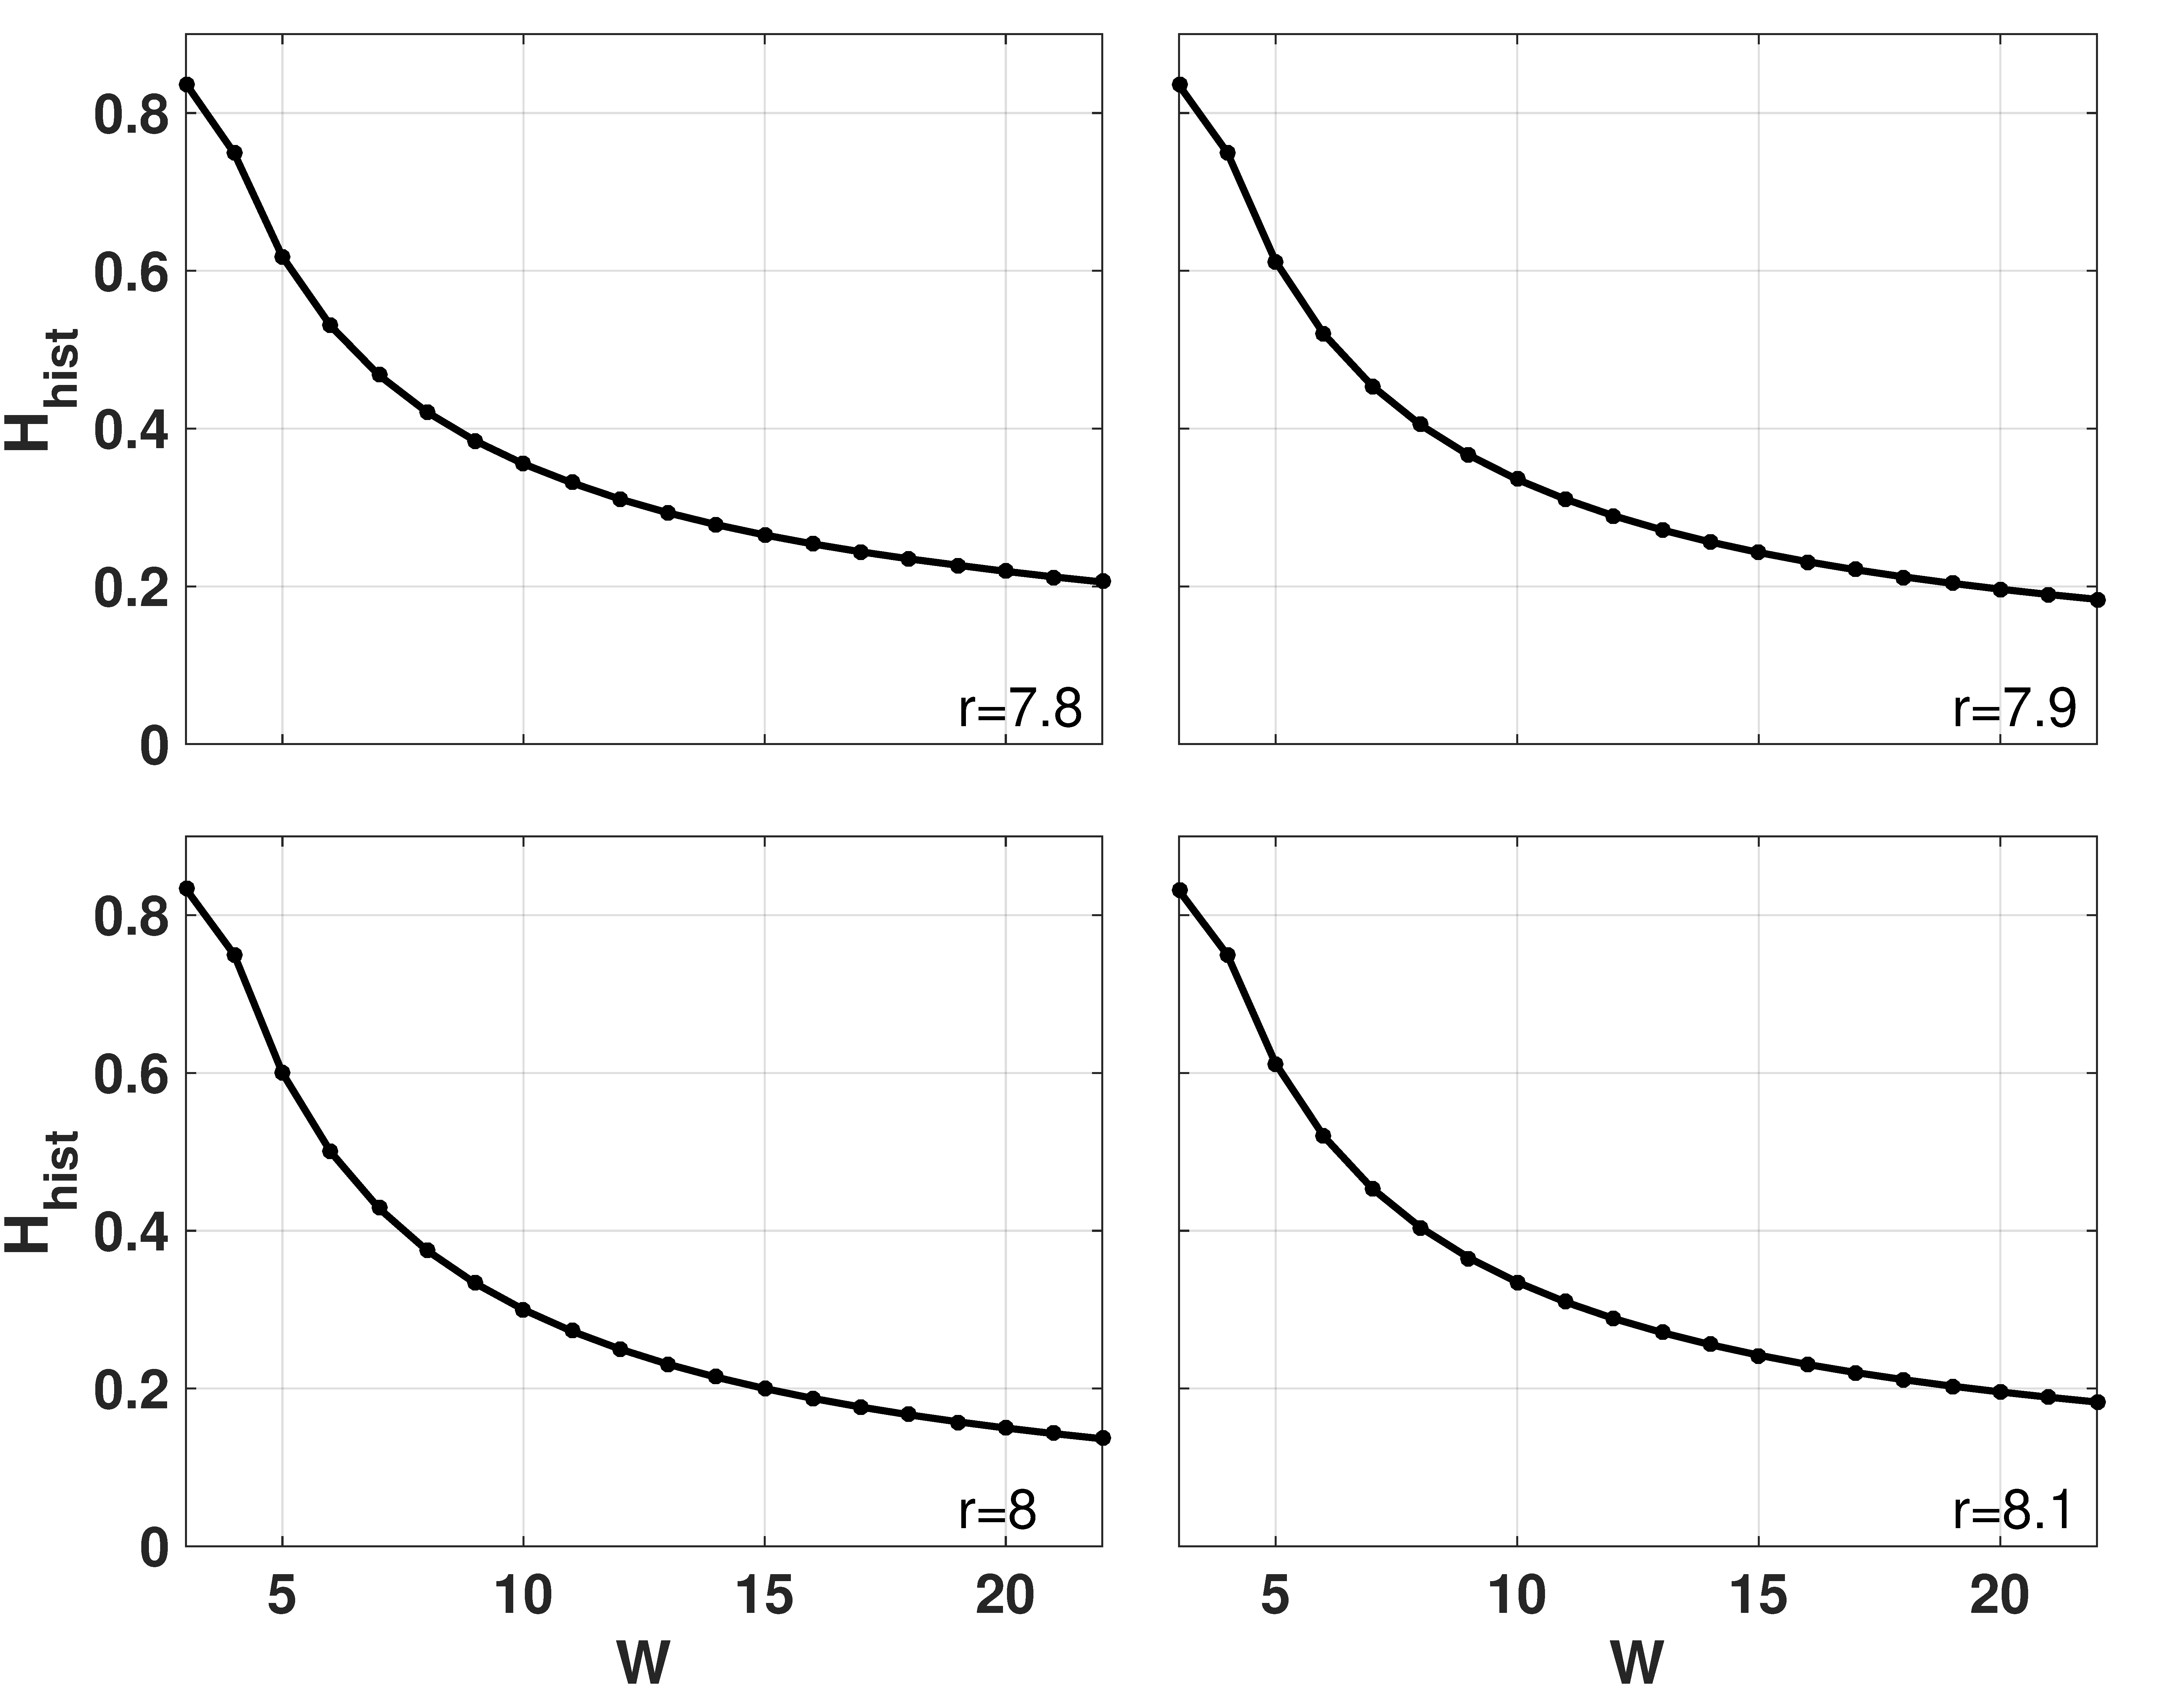
\includegraphics[width=0.8\textwidth]{H_W_rCS}
\caption{Entropía normalizada $H_W$ en función de $W$ para un \emph{RO} sin \textit{jitter} muestreado con diferentes valores de $r$.}
\label{fig:H_W_rCS}
\end{figure}
%
\begin{figure}
\centering
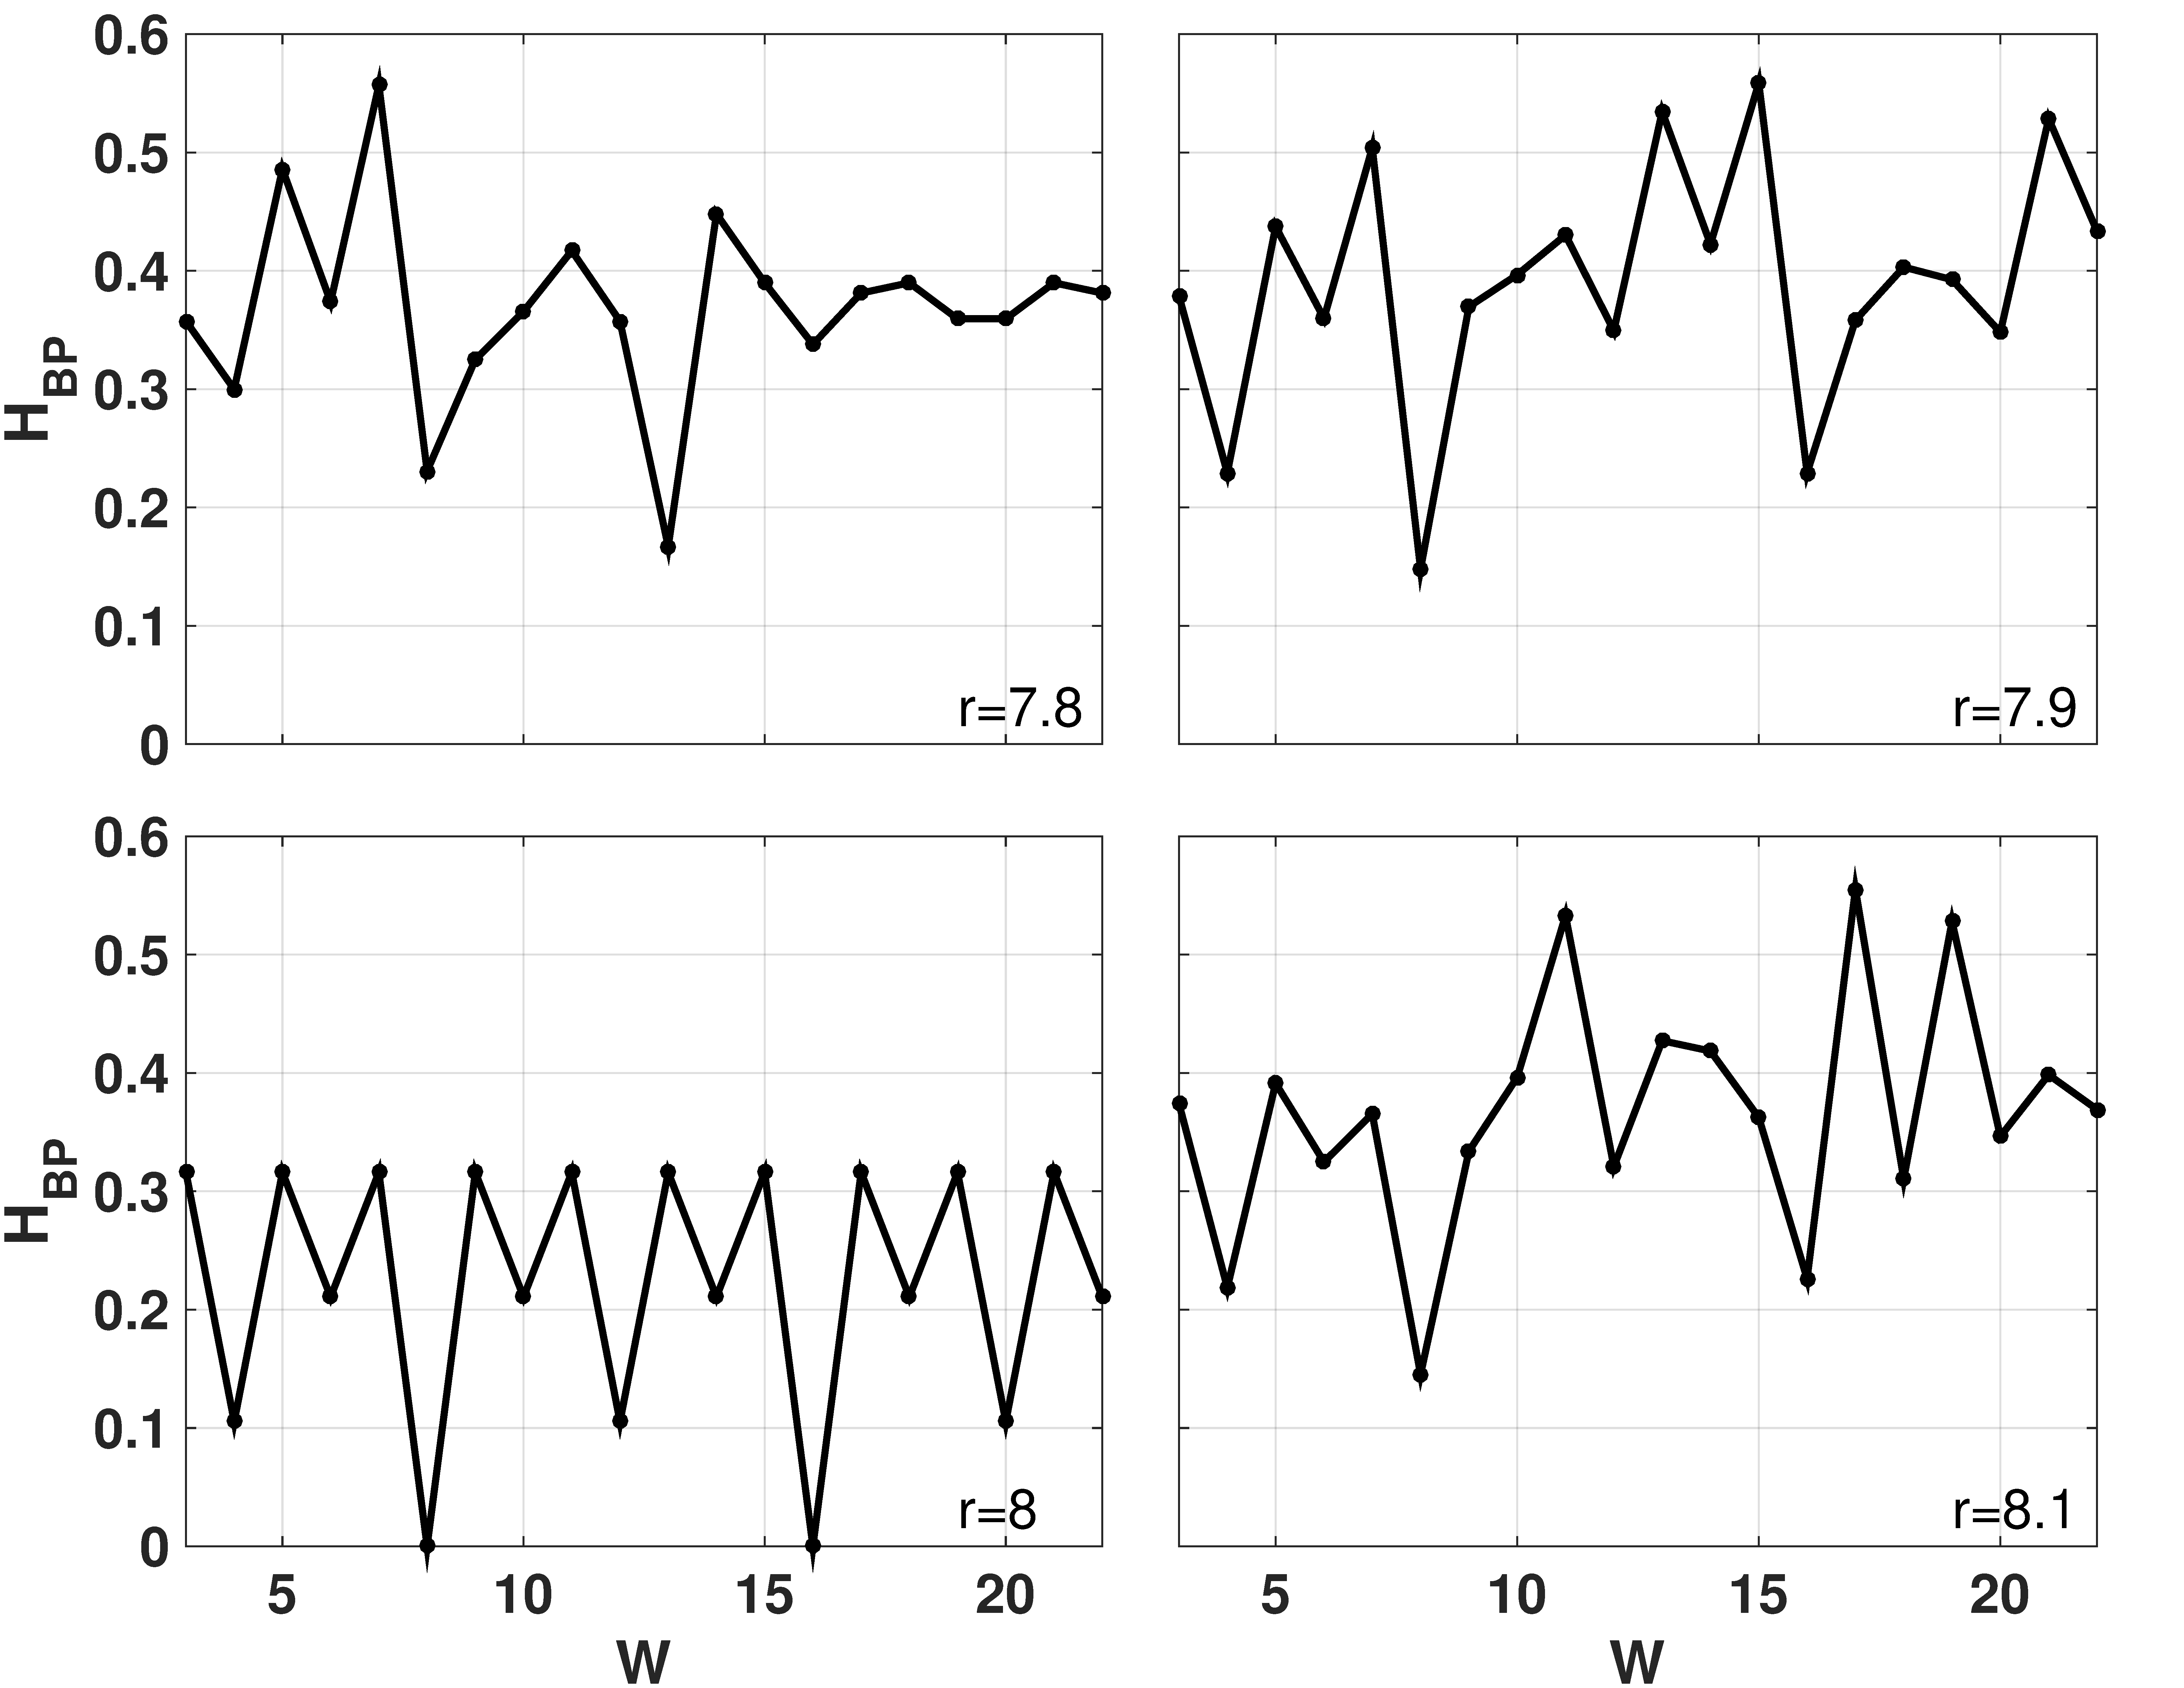
\includegraphics[ width=0.8\textwidth]{HBP_W_rSS}
\caption{$H^{(D)}_{BP}$ en función de  $W$ para un \emph{RO} sin \textit{jitter} muestreado con diferentes valores de $r$. Los cálculos fueron hechos con superposición de palabras}
\label{fig:HBP_W_rSS}
\end{figure}

Estos resultados muestran que los dos cuantificadores, $h$ y $h^*$, son apropiados para ser usados como medidores de \textit{jitter} debido a que: 
\begin{itemize} 
\item (a) Para $\sigma_T=0$ (salida sin \textit{jitter}) se acercan rápidamente a un valor límite constante ya que tanto $D$ como $W$ tienden a $\infty$ y este valor es independiente de $D$ y $W$; 
\item (b) Son funciones monótonas y proporcionales de $\sigma_T$.
\item (c) A partir de su análisis, es posible detectar el valor óptimo de la relación de muestreo $r$.
En las siguientes Figuras se muestran estas afirmaciones que son representativas de todos los resultados presentados.
\end{itemize}
%
La Figura \ref{fig:hm_D_SJ} muestra la entropía diferencial de Bandt \& Pompe $h^*$, como función de $D$, con $W$ como parámetro, para un \textit{RO} sin \textit{jitter}.
Se puede ver que existe un valor umbral $W = 4$ sobre el cual todas las curvas colapsan independientemente del valor de $D$.
Además, la Figura \ref{fig:hm_D_SJ} también muestra que para $D \ge 8$ todas las curvas colapsan, independientemente del valor de $W$.
En conclusión, si $D \ge 8$ y $W \ge 4$ se obtiene un cuantificador independiente de $D$ y $W$.
%
\begin{figure}
	\centering
	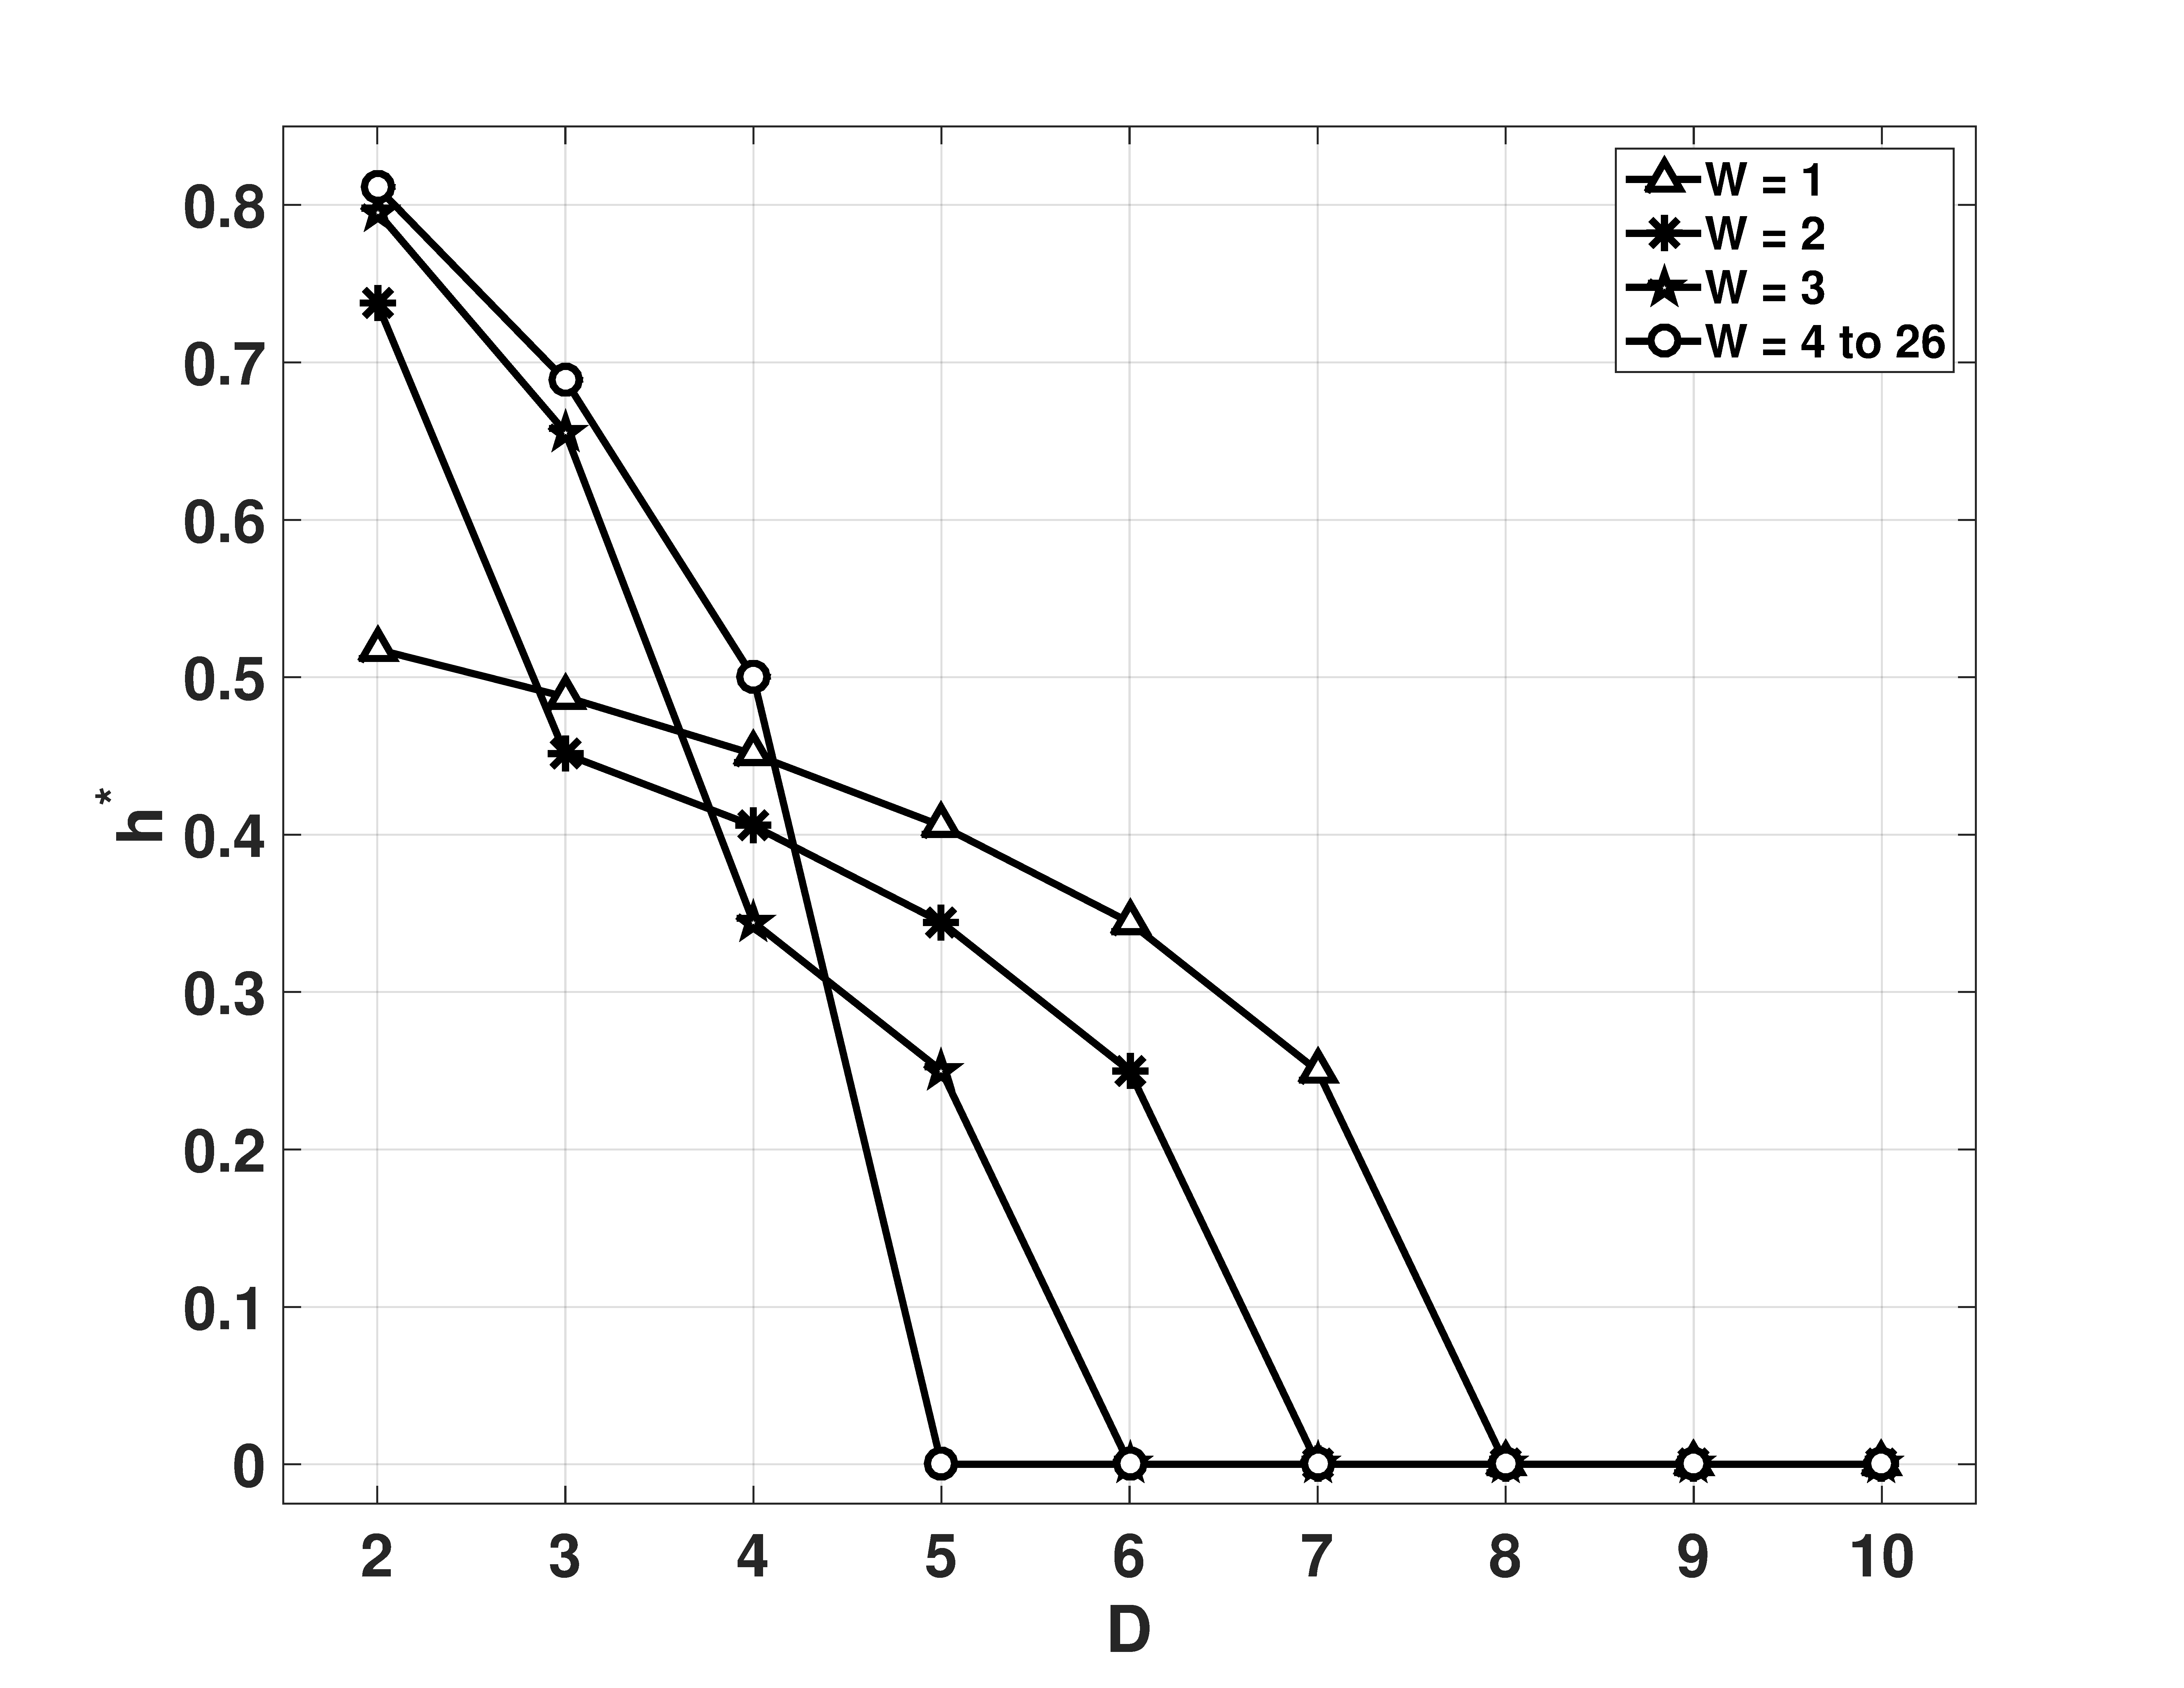
\includegraphics[ width=0.8\textwidth]{hm_D_SJ}
	\caption{$h^*$ en función de $D$ para un \emph{RO} sin \textit{jitter} muestreado con $r=8$.}
	\label{fig:hm_D_SJ}
\end{figure}

La influencia del \textit{jitter} en este cuantificador se muestra en la Figura \ref{fig:hm_D_CJ}, donde $h^*$ se representa como una función de $D$ con $\sigma_T$ como parámetro.
Los valores considerados son $\sigma_T=\{0 (sin~jitter),$ $0.001,$ $0.002,$ $0.003,$ $0.004,$ $0.005,$ $0.007,$ $0.01,$ $0.02,$ $0.02,$ $0.04,$ $0.05,$ $0.07,$ $0.1\}$.
El recuadro de la Figura \ref{fig:hm_D_CJ} muestra $h^*$ como función de $\sigma_T$ para $D = 8$.
Este recuadro muestra que $h^*$ es una función monótona creciente de $\sigma_T$.
%
\begin{figure}
	\centering
	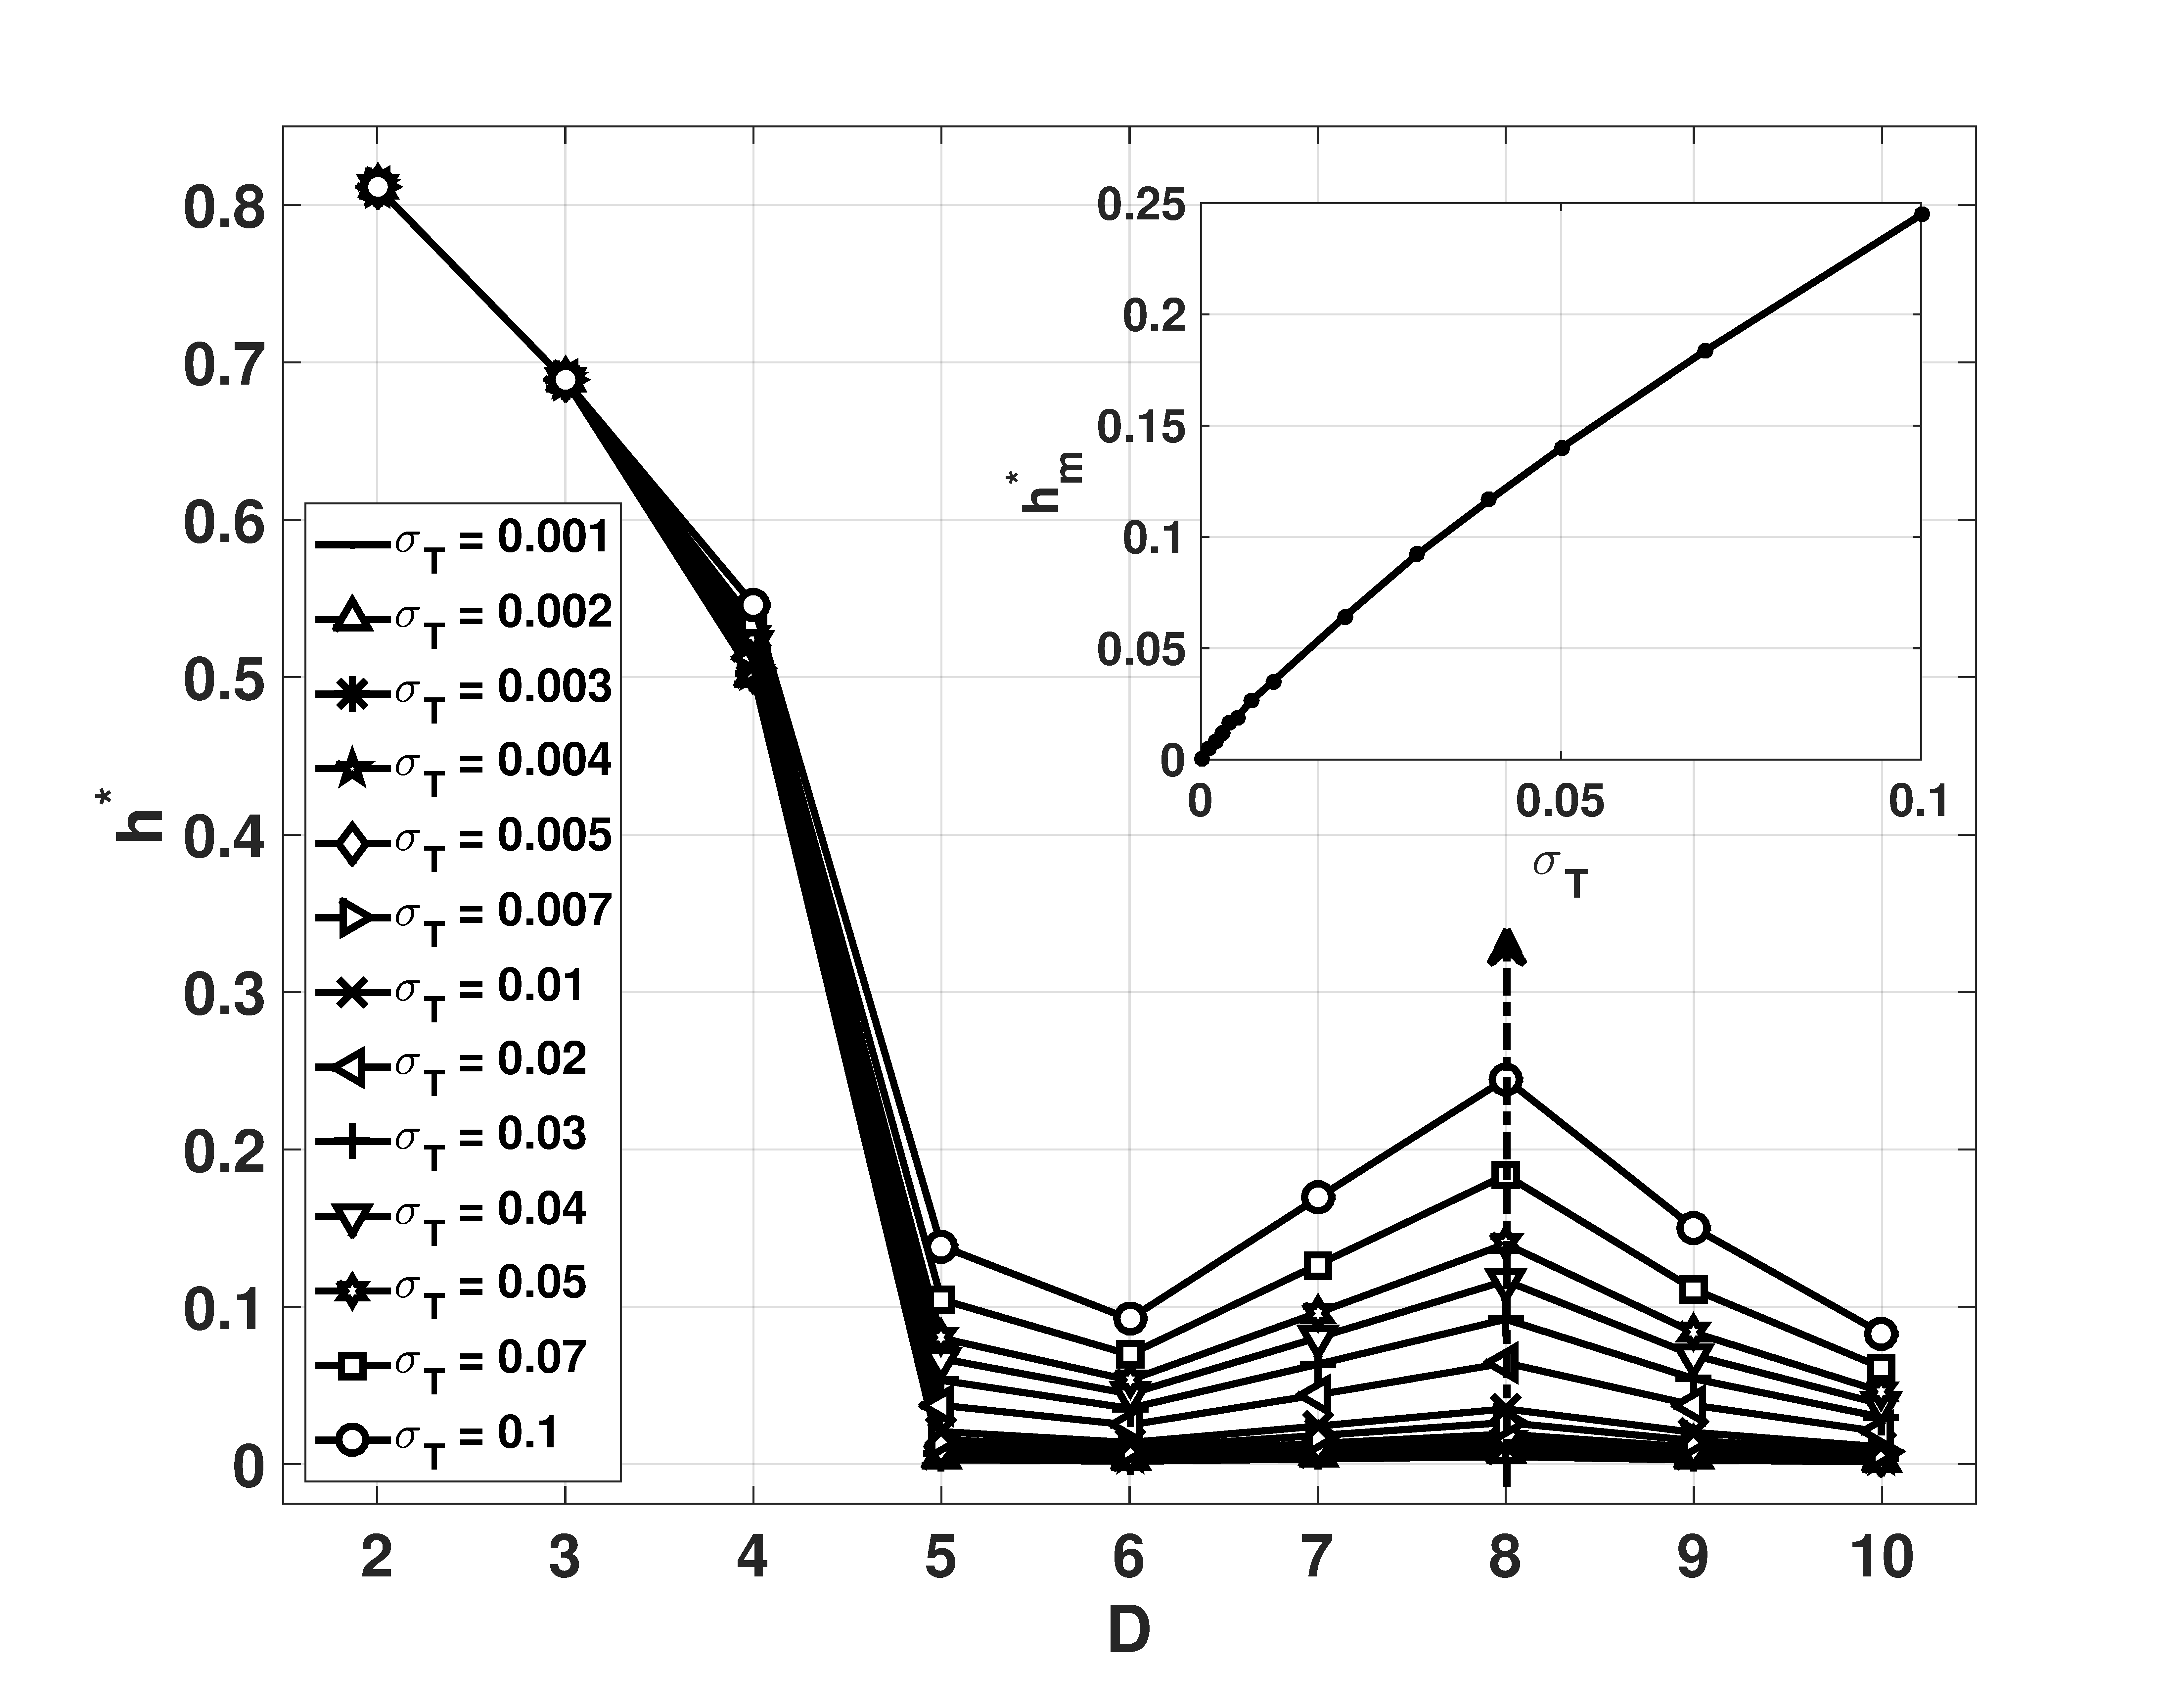
\includegraphics[width=0.8\textwidth]{hm_D_CJ}
	\caption{$h^*$ en función de $D$ para un \emph{RO} muestreado con $r=8$ con longitud de palabra $W=6$ para \textit{jitter} con diferentes varianzas. El recuadro muestra $h^*$ en función de $\sigma_T$ para $r=8$, $W=6$ y $D=8$.}
	\label{fig:hm_D_CJ}
\end{figure}

Finalmente, la Figura \ref{fig:hm_r_CJ} muestra $h^*$ como una función de la relación de muestreo $r$.
En esta Figura, se muestra que hay un mínimo para el $r$ correcto (en este caso $r = 8$).
Además, la sensibilidad de $h^*$ en función del \textit{jitter} es máxima para este mismo valor ideal de $r$.
%
\begin{figure}
\centering
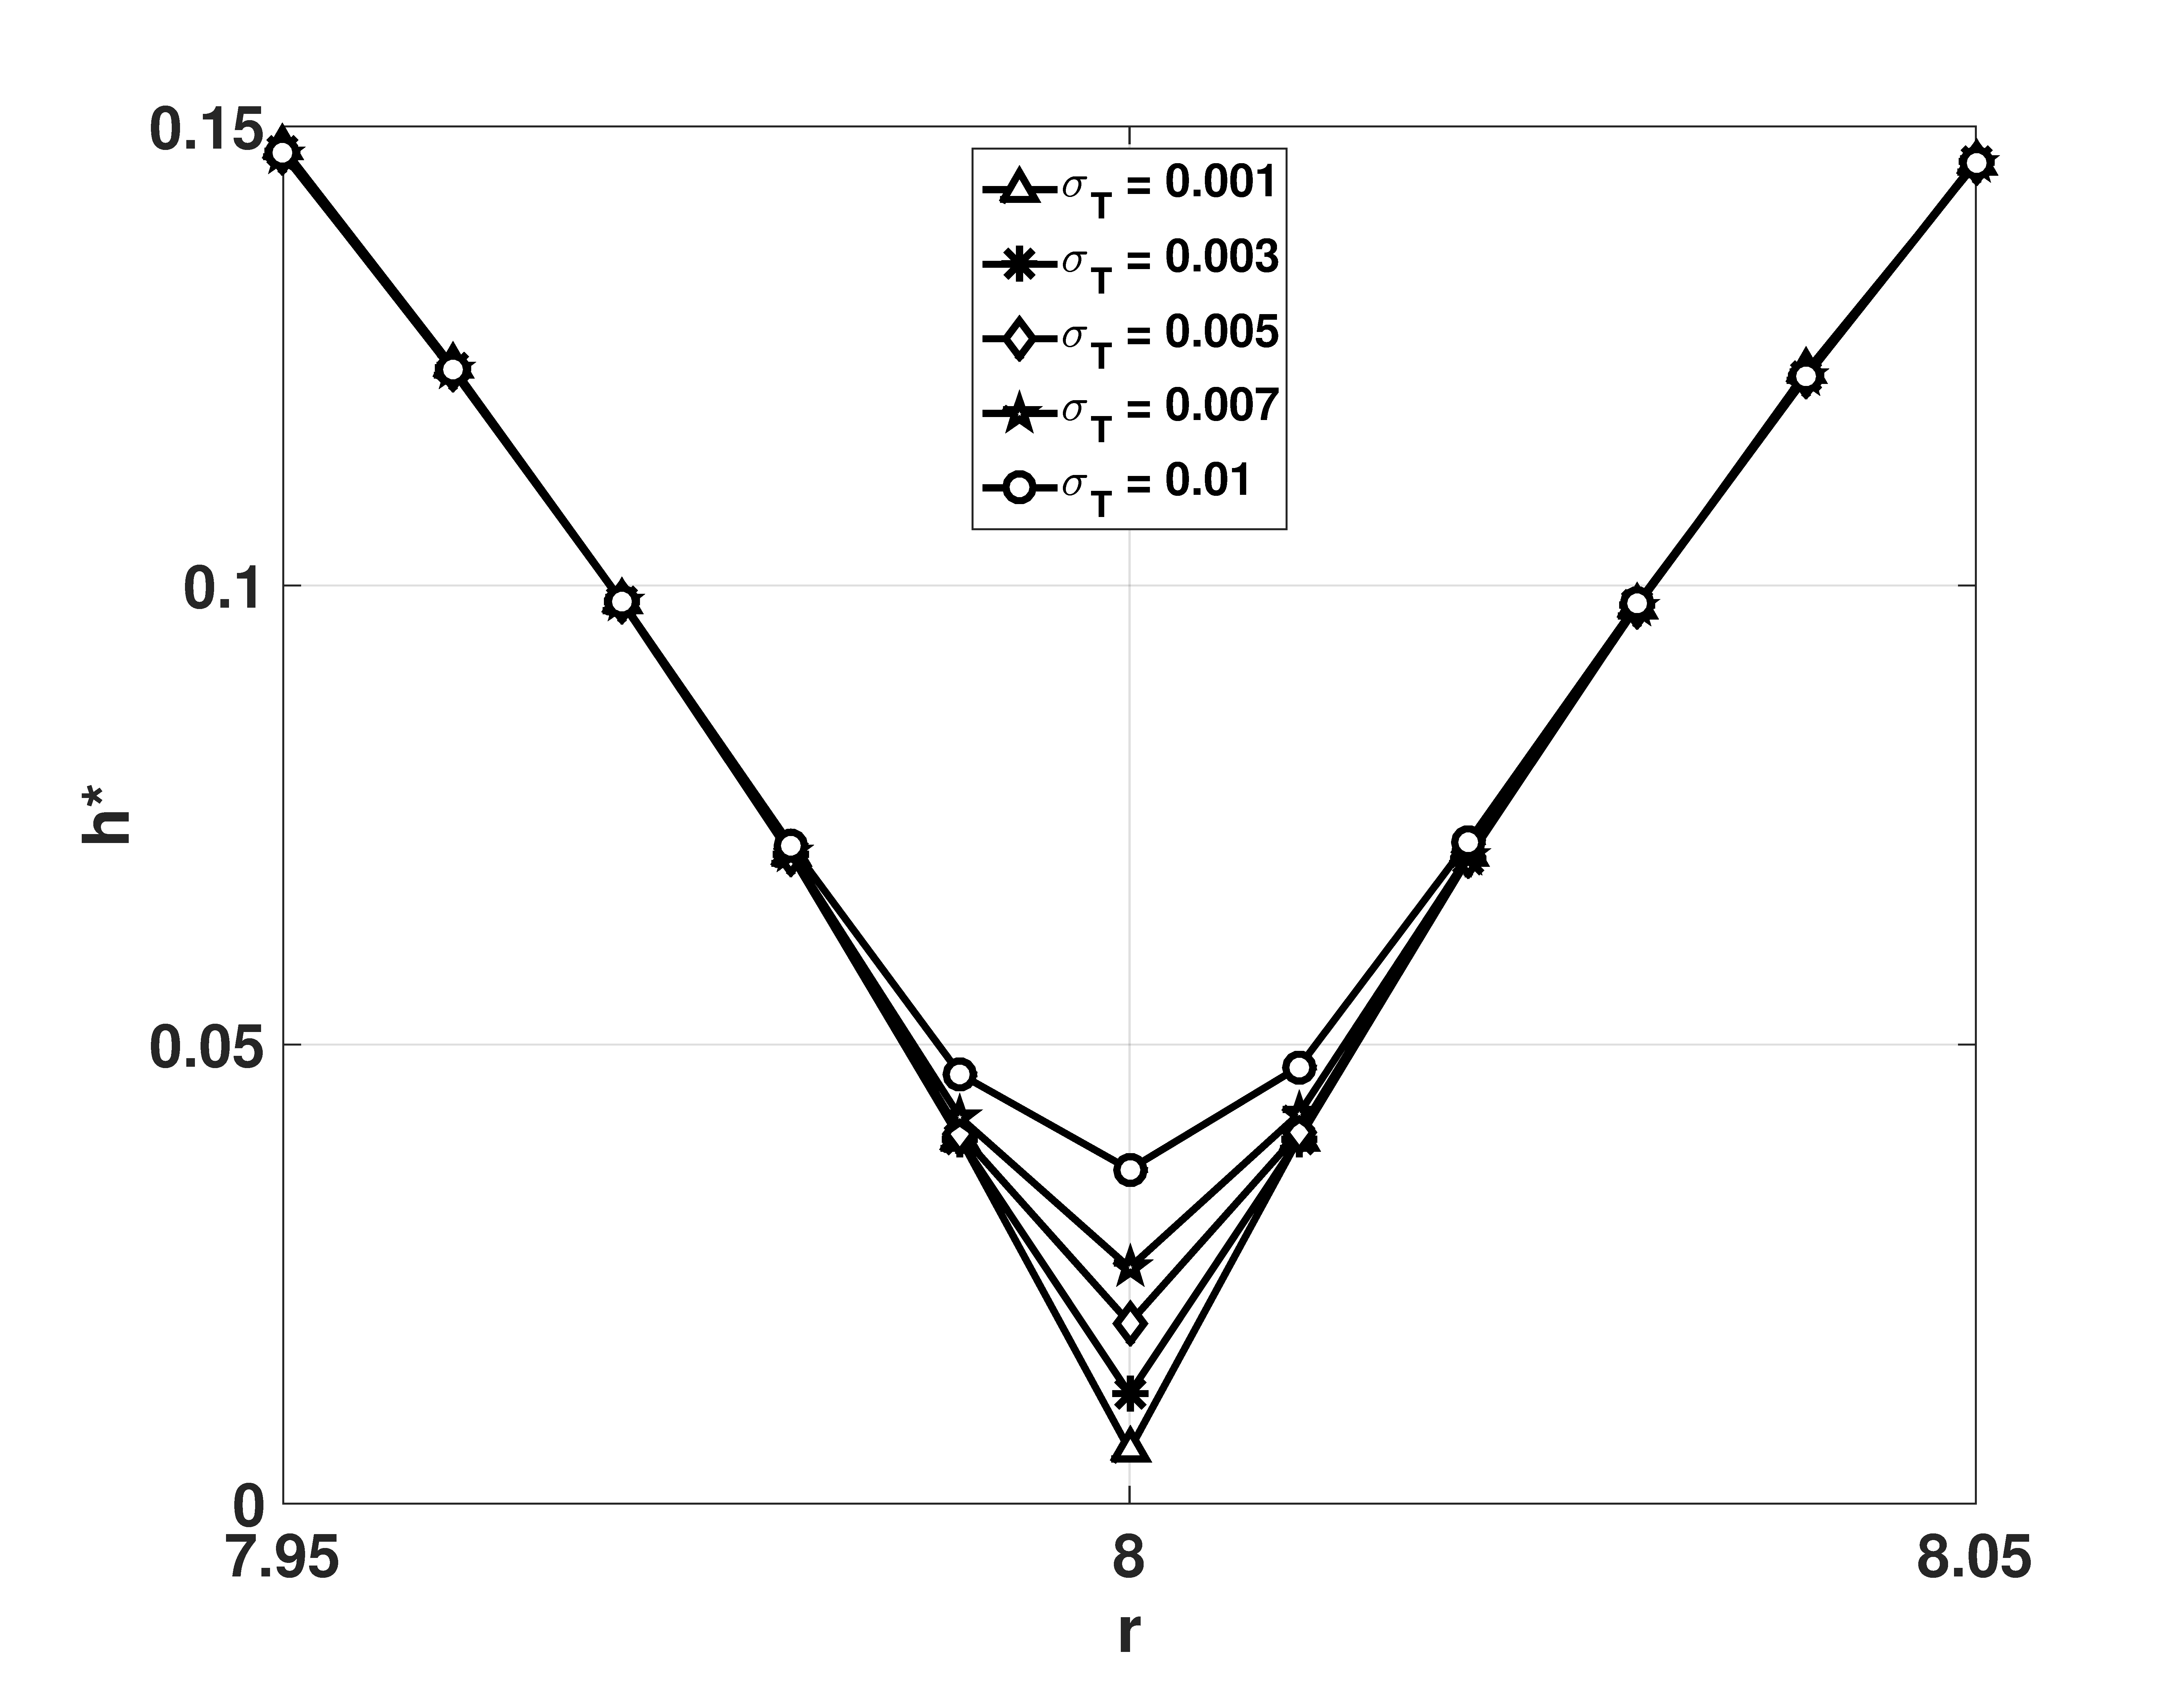
\includegraphics[ width=0.8\textwidth]{hm_r_CJ}
\caption{$h^*$ en función de $r$ para $r\in[7.95,8.05]$, con algunos $\sigma_T$, $W=6$ y $D=8$. La curva tiene un mínimo en el valor correcto de $r=8$.}
\label{fig:hm_r_CJ}
\end{figure}

En cuanto al segundo cuantificador $h$, se observa que sólo depende de $W$ ya que el parámetro $ D $ no se usa para definir la \emph{PDF} asignada a la serie de datos.
La Figura \ref{fig:h_W_SJ} muestra un caso sin \textit{jitter}, $h$ es independiente de $W$ para $W \ge 4$.
Para lo siguiente se adoptó $W = 6$.
%
\begin{figure}
	\centering
	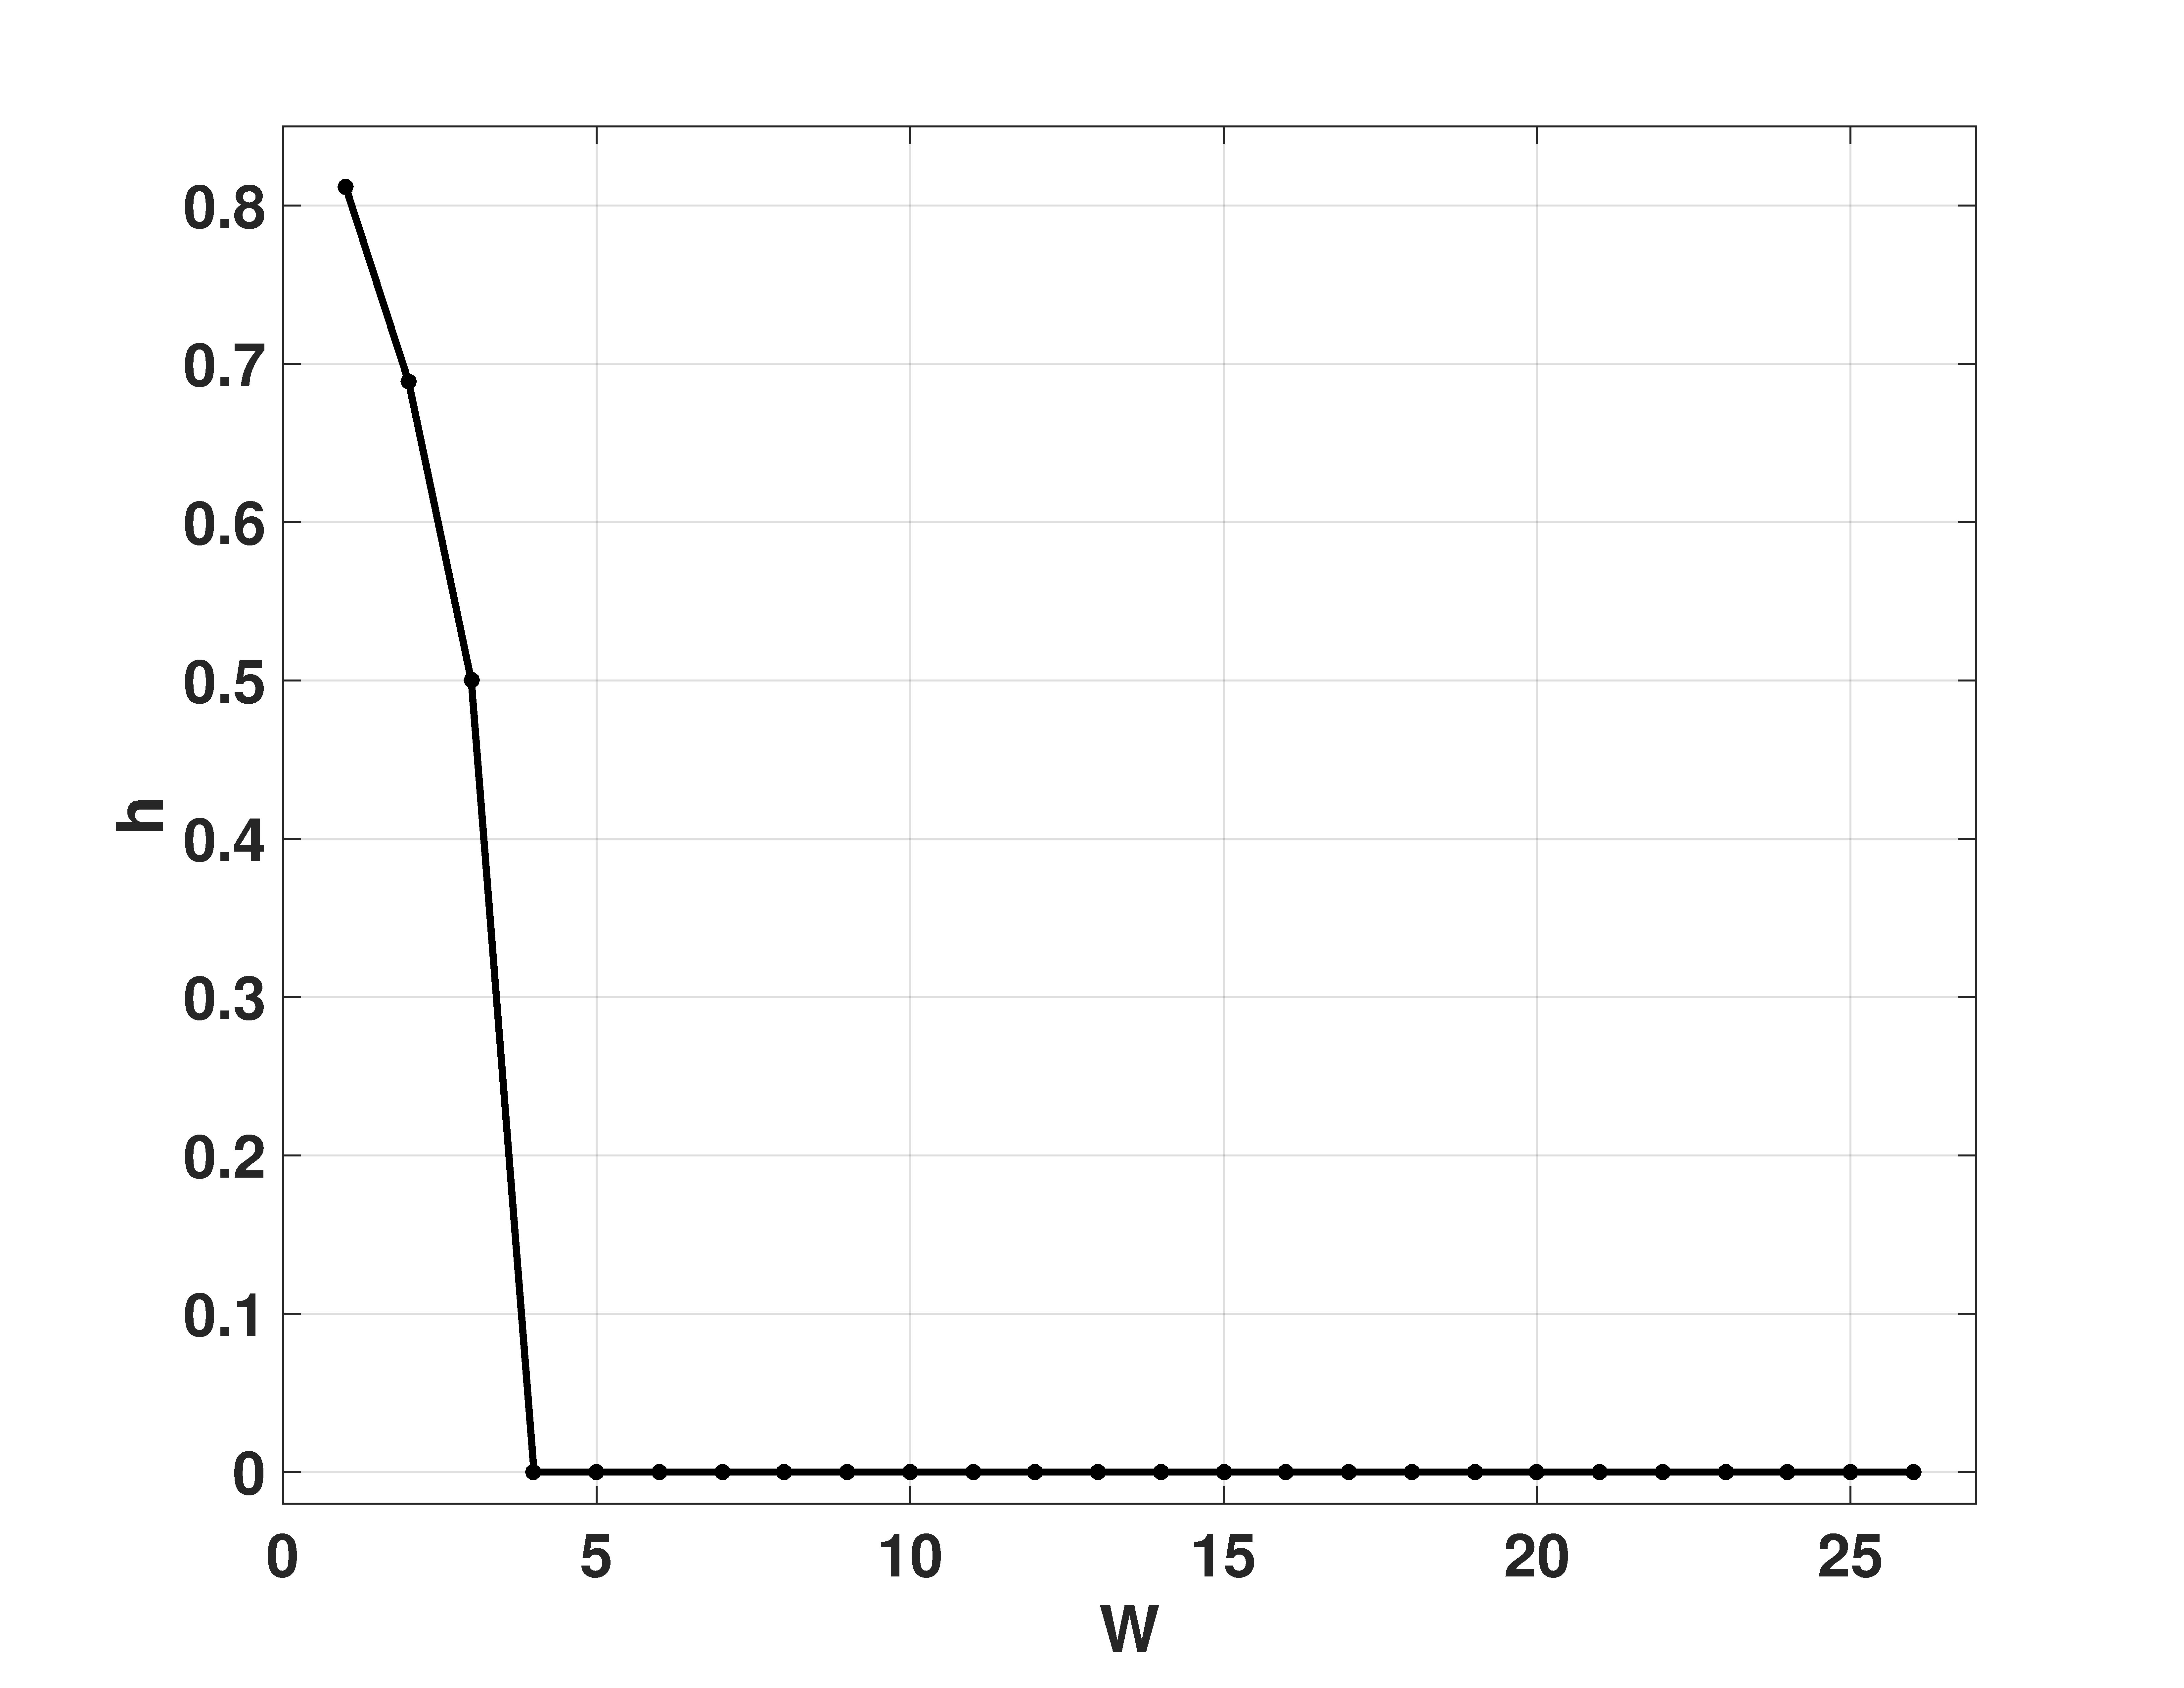
\includegraphics[width=0.8\textwidth]{h_W_SJ}
	\caption{$h$ en función de $W$ para un \emph{RO} sin \textit{jitter} muestreado con $r=8$.}
	\label{fig:h_W_SJ}
\end{figure}

La Figura \ref{fig:h_W_CJ} muestra la influencia del \textit{jitter} sobre este cuantificador.
Queda claro en el recuadro de esta Figura que, para el valor seleccionado $W = 6$, $h$ es una función monótona creciente de la varianza del \textit{jitter} $\sigma_T$.
%
\begin{figure}
	\centering
	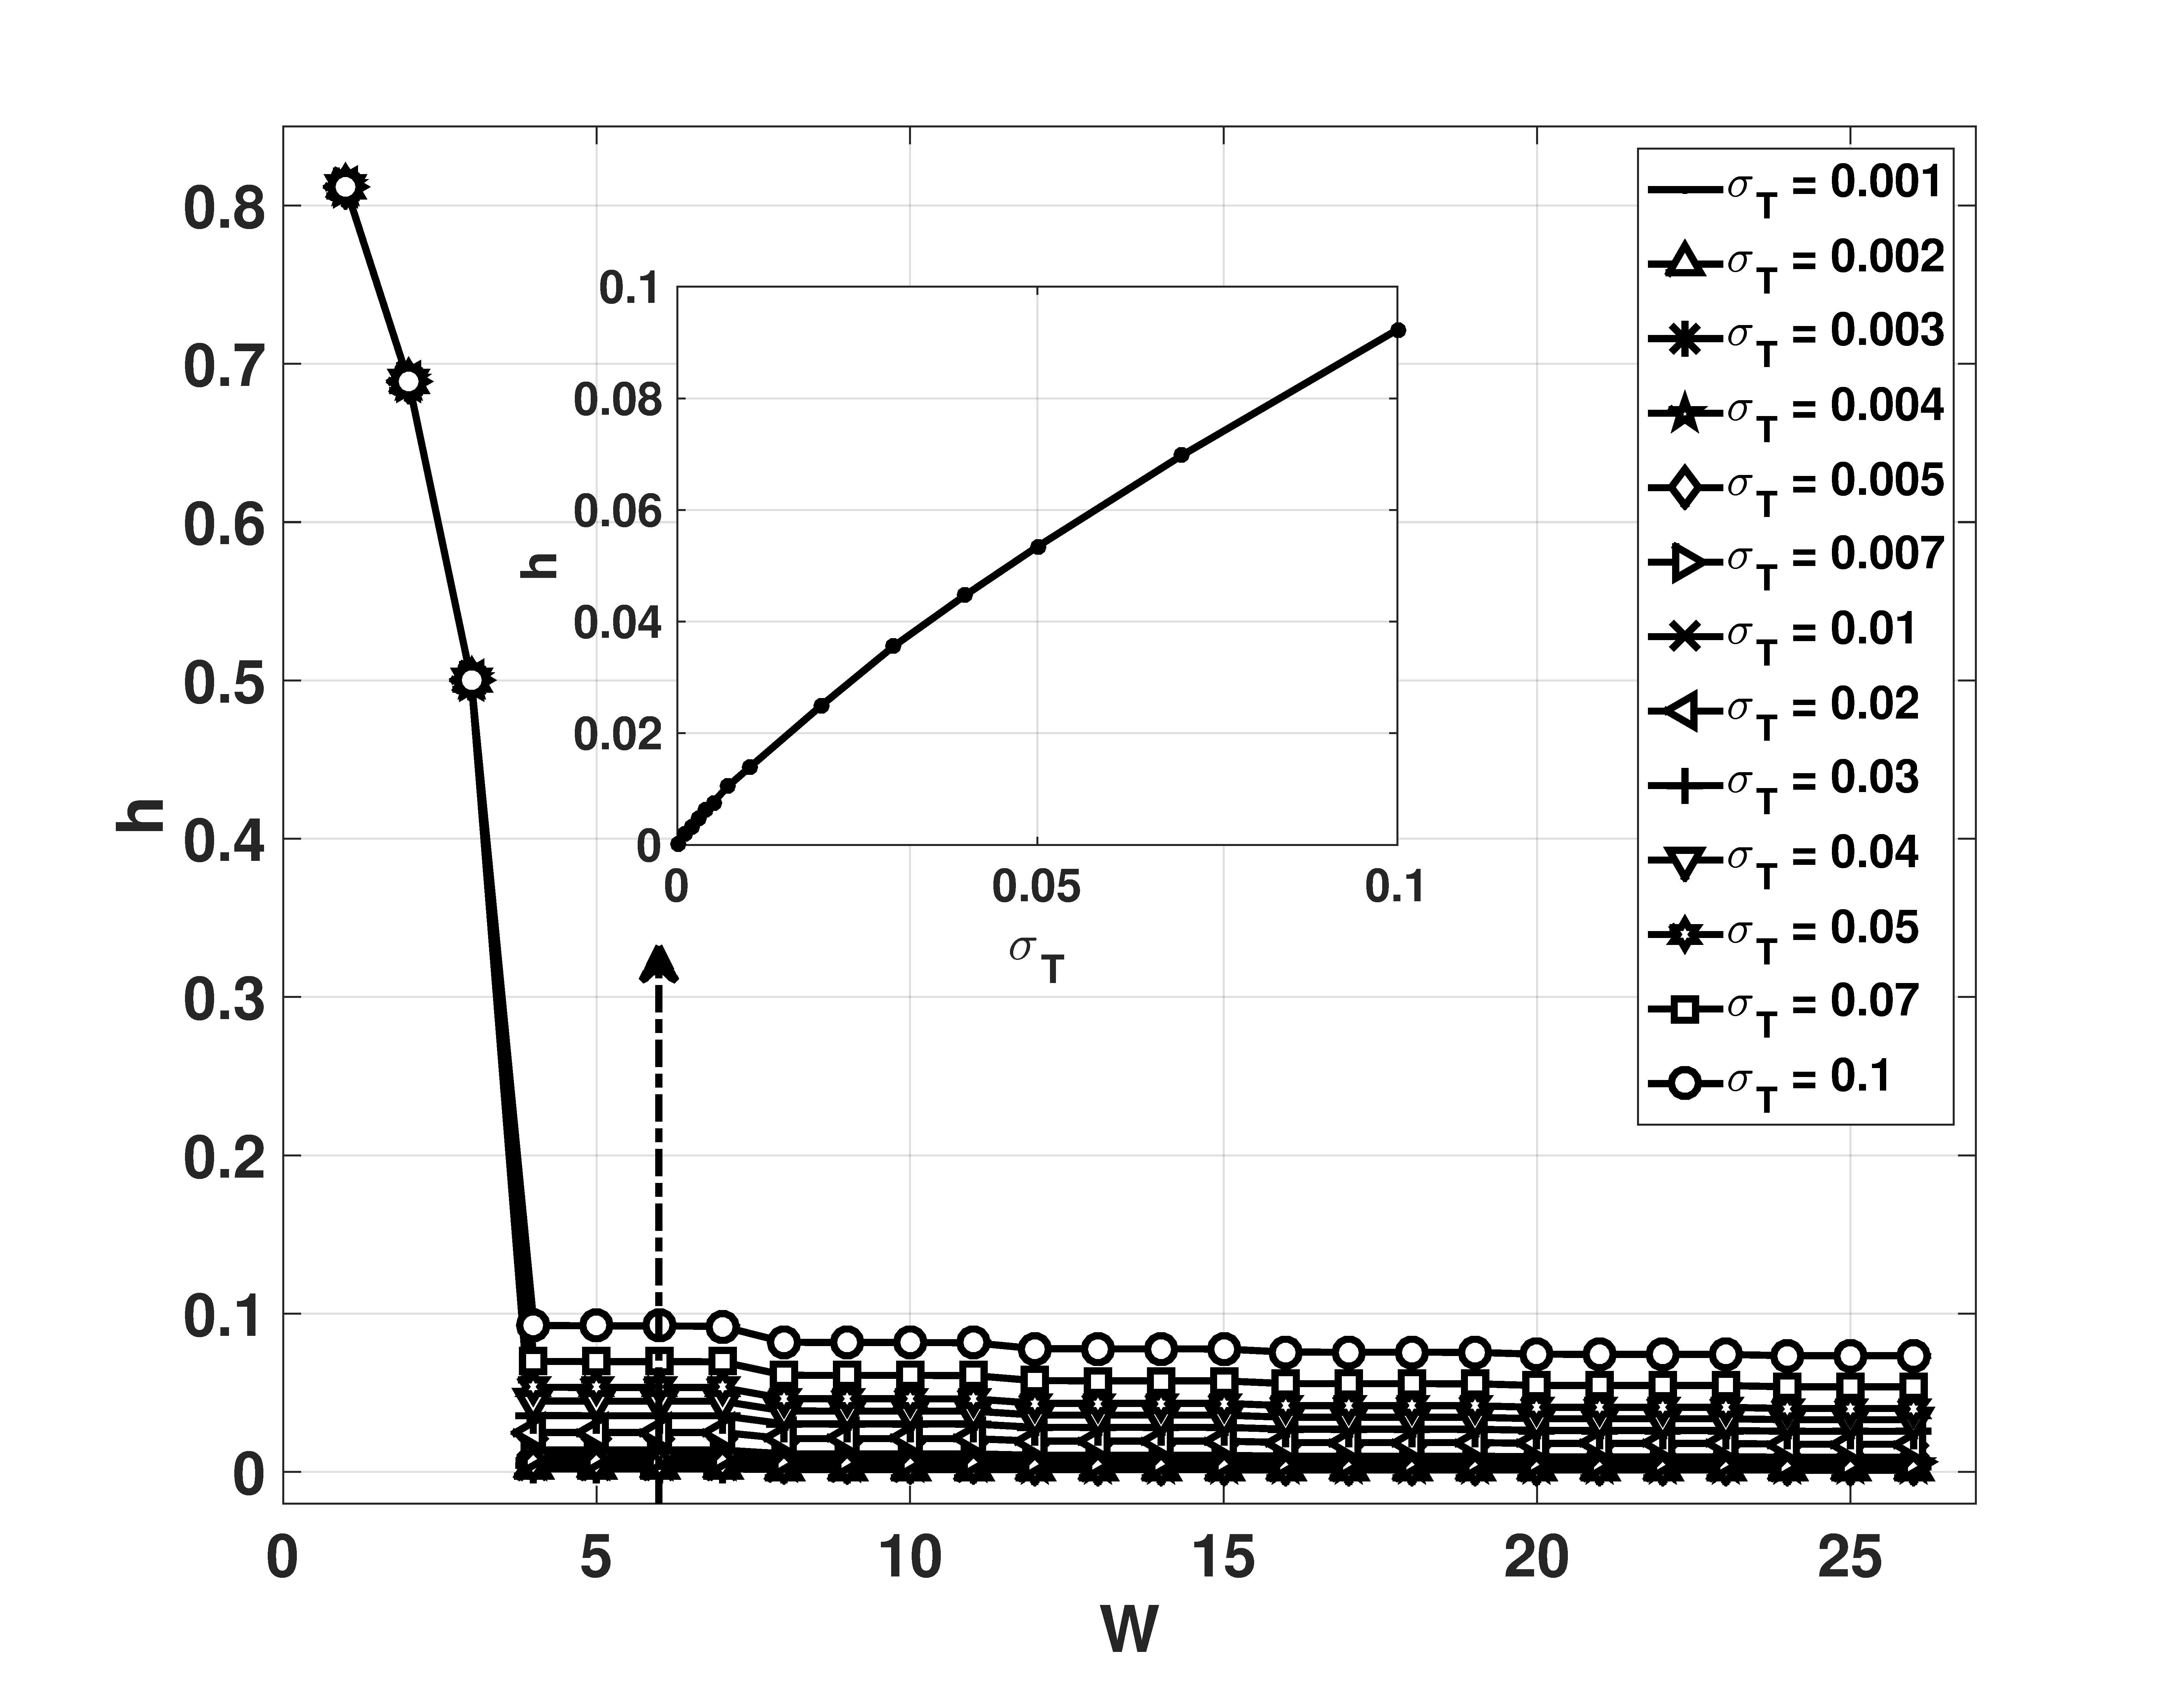
\includegraphics[ width=0.8\textwidth]{h_W_CJ}
	\caption{$h$ en función de $W$ para un \emph{RO} muestreado con $r=8$, con \textit{jitter} con distintas varianzas. El recuadro muestra $h$ en función de $\sigma_T$ con $r=8$ y $W=6$.}
	\label{fig:h_W_CJ}
\end{figure}

La Figura \ref{fig:h_r_CJ} muestra que $h$ tiene un mínimo cuando $r$ toma su valor óptimo ($r = 8$).
Cabe destacar que este mínimo es robusto también en presencia de jitter.
%
\begin{figure}
\centering
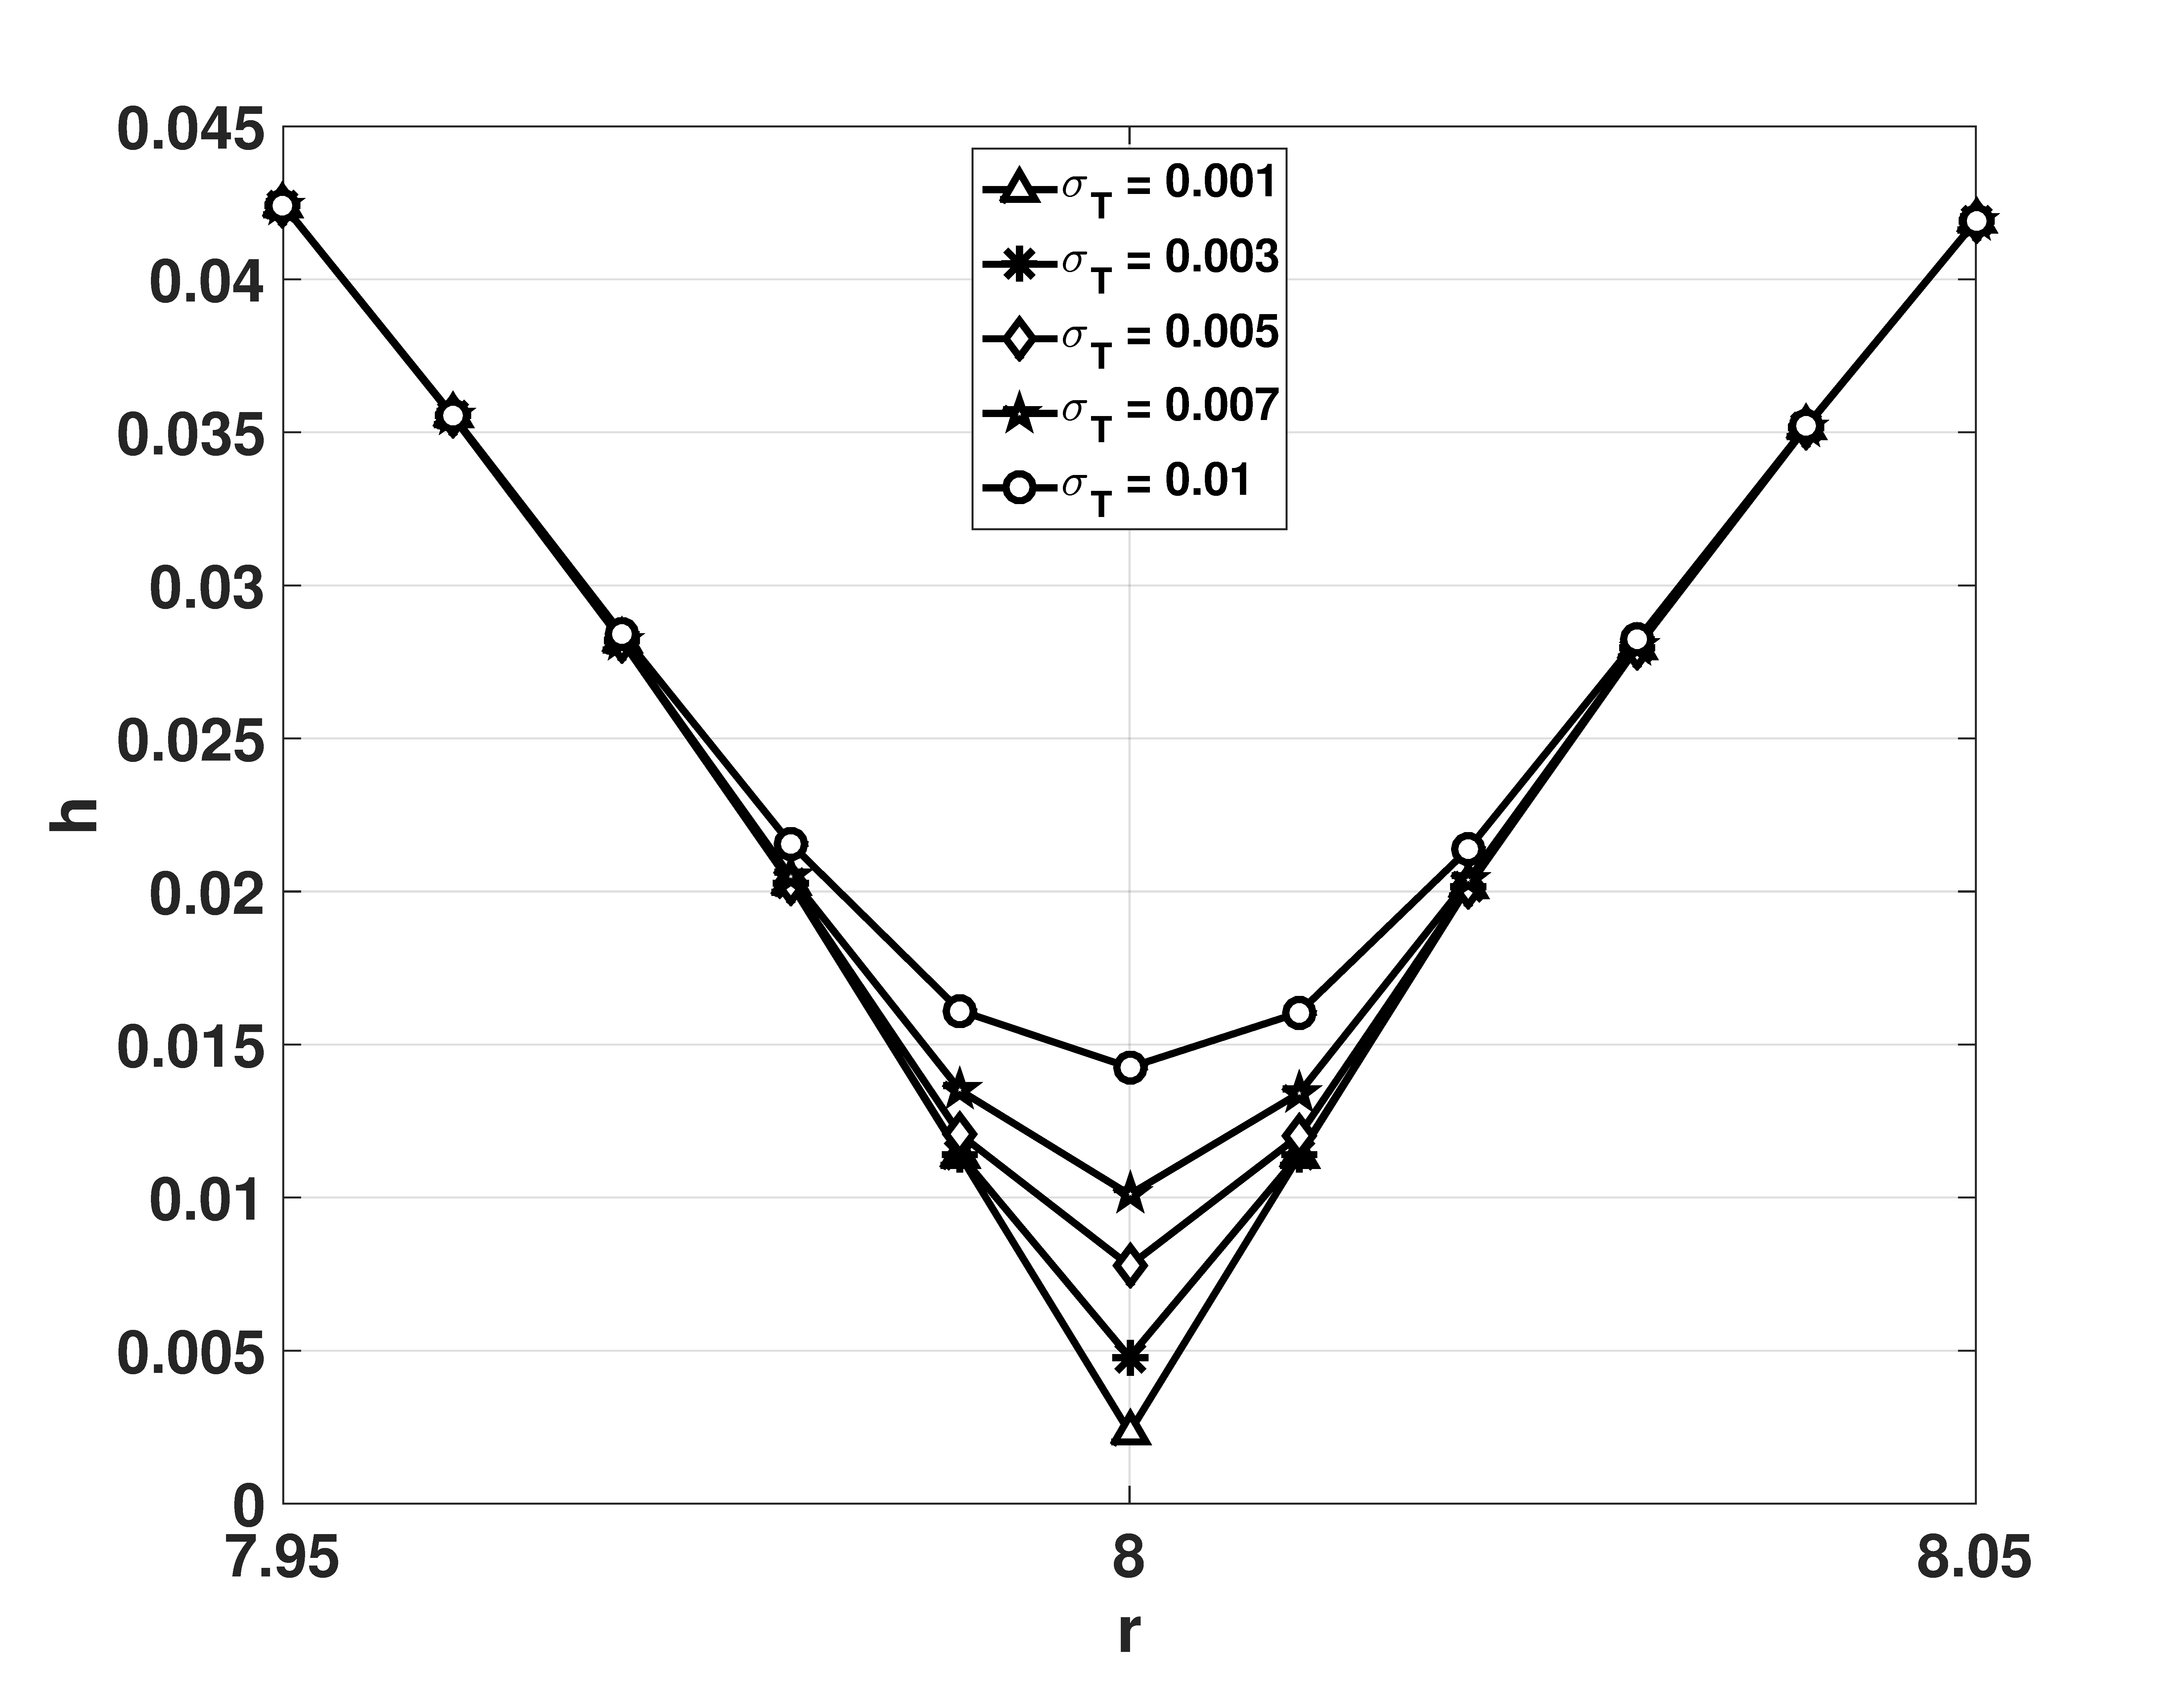
\includegraphics[ width=0.8\textwidth]{h_r_CJ}
\caption{$h$ en función de $r$ con $r\in[7.95,8.05]$, para distintos $\sigma_T$ y $W=6$ . La curva tiene un mínimo en $r=8$.}
\label{fig:h_r_CJ}
\end{figure}

Se debe realizar un análisis adicional para asegurar que al utilizar los valores seleccionados $W = 6$ y $D = 8$ se este trabajando con una cantidad de datos suficiente para tener una buena estadística.
De acuerdo con la Sección \ref{capCuanti}, para un alfabeto dado $\mathcal{A}$ con $m$ elementos, y un archivo simbólico dado de longitud $n$, se define el parámetro de calidad $\alpha = n/m$.
La calidad es mejor a medida que $\alpha$ aumenta y para esta aplicación se acepta un valor mínimo $\alpha = 10$.
Los valores seleccionados $W = 6$ y $D = 8$ proporcionan $\alpha_h \simeq 10^5$, $ \alpha_ {h^*} \simeq 175$ si las $w_i$ palabras son tomadas con superposición.
Si las palabras son tomadas con superposición, resulta $ \alpha_ {h^*} \simeq 29$.
Todos los casos se trabajó con un valor $\alpha>10$ como es requerido.

La Figura \ref{fig:hm_h_CJ} muestra el plano $h^*_{m} \times h$.
Los cuantificadores se calcularon barriendo los valores de $D$ de $2$ a $11$ y $W$ de $2$ a $26$ (se barrió ambos para $h^*$ y sólo $W$ en el caso de $h_{hist}$).
Se obtuvo una mejor diferenciación para valores más altos de los parámetros, esto se debe a que ambos cuantificadores tienden a cuantificar la entropía de la fuente cuando $D$ y $W$ tienden a infinito.
Sin embargo esto es imposible en la práctica real, la cantidad de datos disponibles limita los valores de los parámetros para lograr buenas estadísticas.
Por lo tanto, se buscaron los valores mínimos (valor umbral) de los parámetros que distinguieran suficientemente bien el \textit{jitter}.
%
\begin{figure}
	\centering
	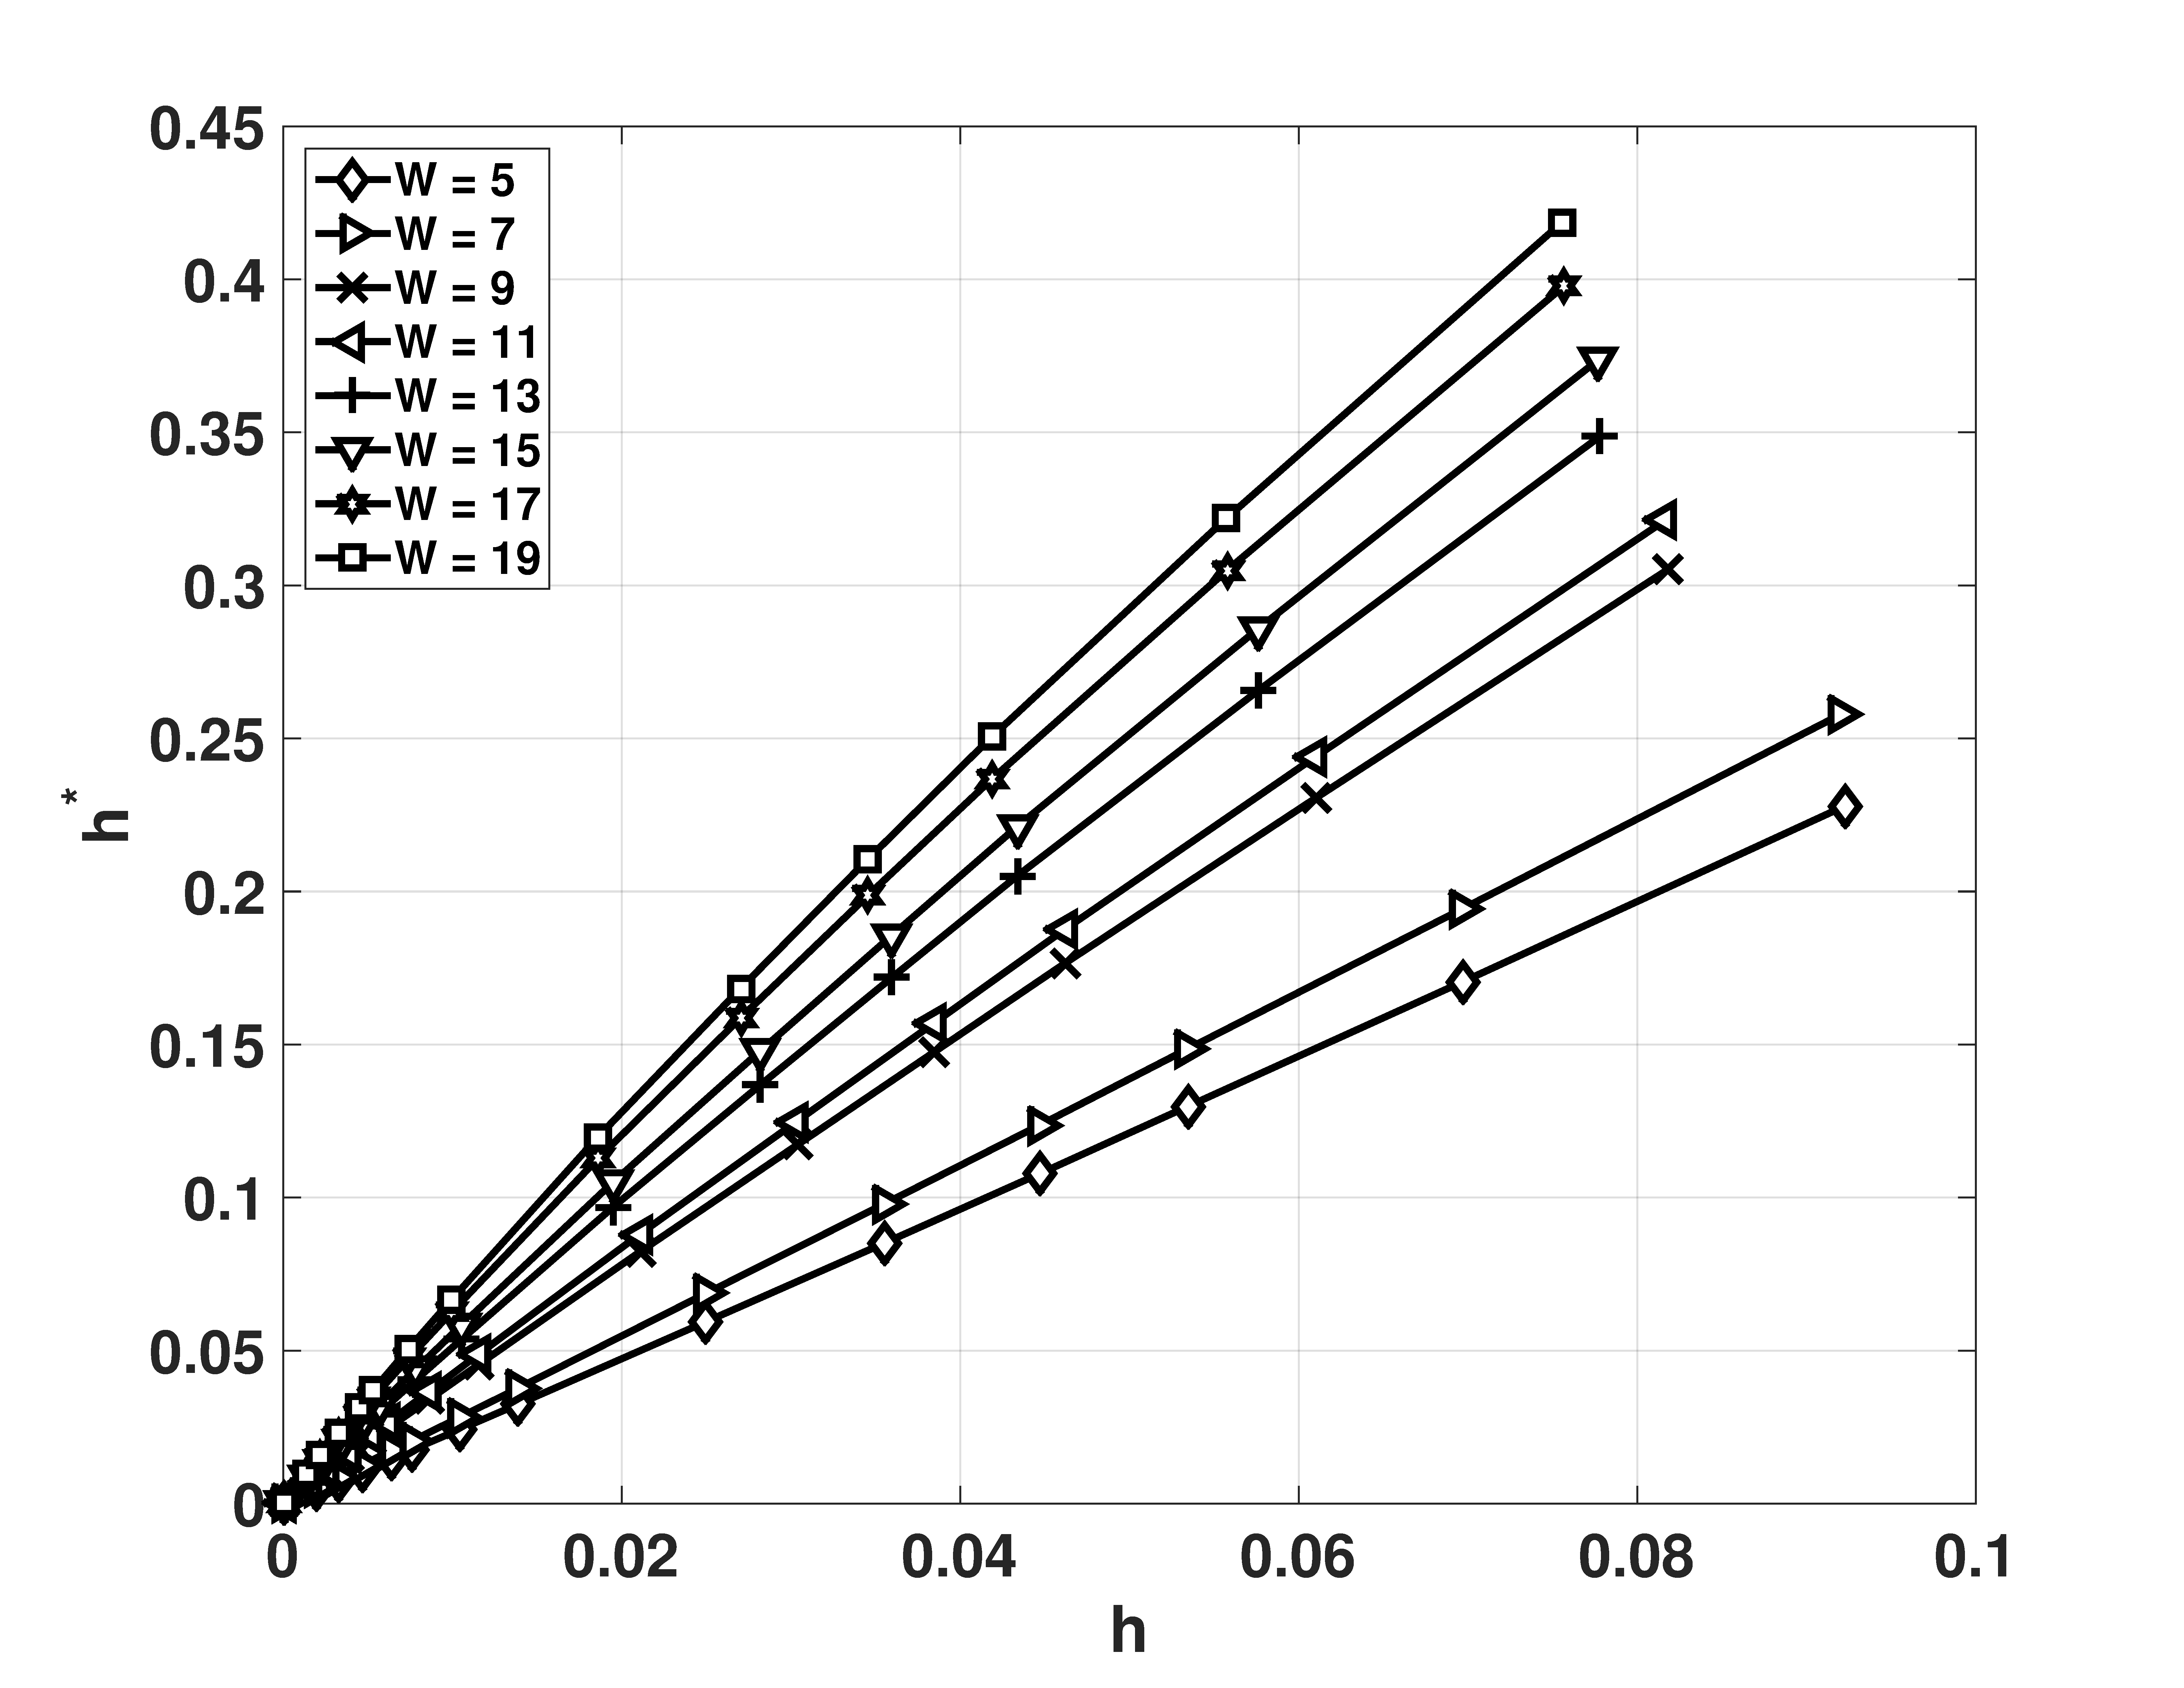
\includegraphics[ width=0.8\textwidth]{hm_h_CJ}
	\caption{$h^*$ como función de $h$ para $r=8$, $D=8$ y diferentes valores de $W$.}
	\label{fig:hm_h_CJ}
\end{figure}

Una comparación entre ambos cuantificadores se muestra en la Figura \ref{fig:hm_h_CJ}.
Los marcadores corresponden a varianzas $\sigma_T=\{0,$ $0.001,$ $0.002,$ $0.003,$ $0.004,$ $0.005,$ $0.007,$ $0.01,$ $0.02,$ $0.03,$ $0.04,$ $0.05,$ $0.07,$ $0.1\}$.
Hay que tener en cuenta que la pendiente de cualquiera de estas curvas es $dh^*/dh$ y es igual al cociente entre las pendientes de curvas en los recuadros de las Figuras \ref{fig:hm_D_CJ}, y \ref{fig:h_W_CJ}.
Si $dh^*/dh\to1$, $h^*$ es más sensible que $h$ para medir el \textit{jitter}.
La pendiente aumenta levemente de $\sim2.47$ para $W =5 $ a $\sim5.54$ para $W = 19$, esto muestra que $h^*$ se vuelve más sensible a medida que aumenta $W$.

También se evaluó $h^*$ sin la superposición de bits entre números naturales consecutivos pero manteniendo la superposición de los $D-1$ números naturales entre patrones de orden (en todos los casos $h$ se evaluó con la superposición de $W-1$ bits consecutivos).
Los resultados se representan en la Figura \ref{fig:Deltahm_Deltah_CS_SS} donde se muestra que al eliminar la superposición aumenta la sensibilidad de este cuantificador.
Por supuesto, se obtiene una cantidad menor de $W$ bits en números naturales del archivo original de siete millones de datos binarios, y en consecuencia, la calidad estadística es menor que la del cálculo original con superposición.
Para aumentar el valor de $\alpha$ hy llegar al minimo nivel requerido y asegurar una buena estadística, se requieren archivos binarios más largos.
%
\begin{figure}
\centering
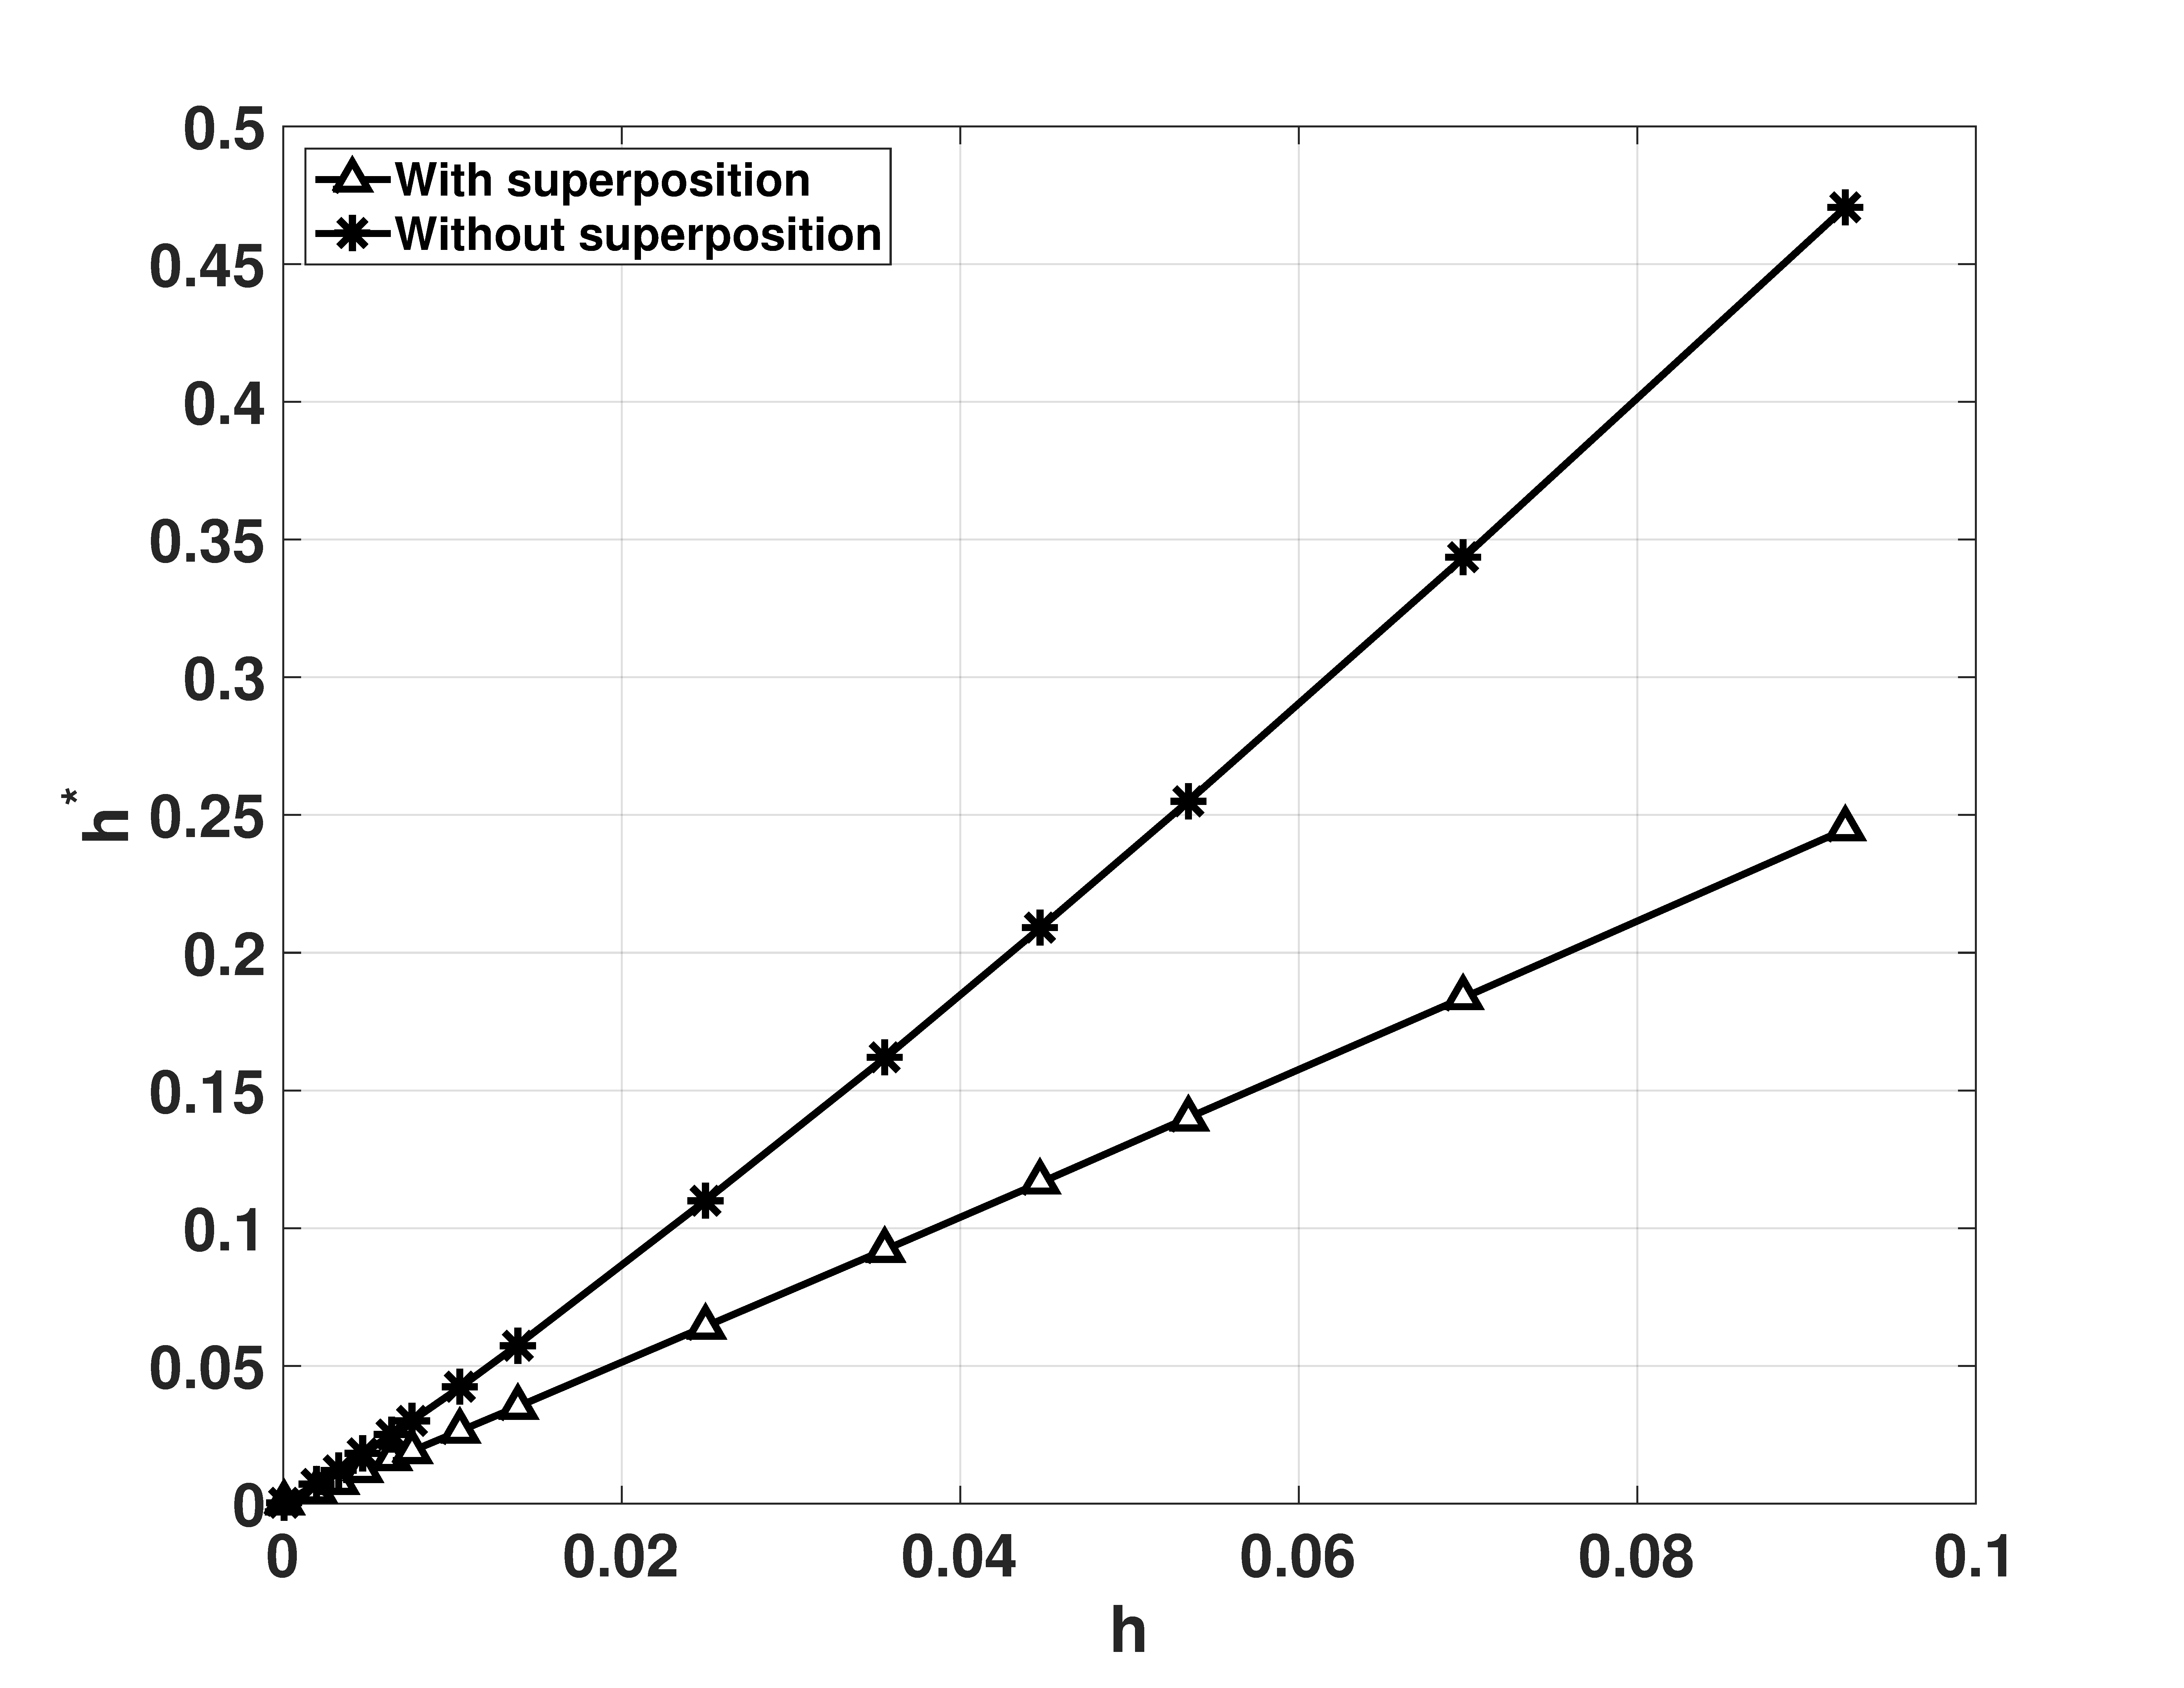
\includegraphics[ width=0.8\textwidth]{Deltahm_Deltah_CS_SS}
\caption{$h^*$ en función de $h$ para $r=8$, $W=6$ y $D=8$. Son considerados los dos procedimientos para obtener números naturales de $W$-bits: con y sin superposición (see text).}
\label{fig:Deltahm_Deltah_CS_SS}
\end{figure}

En la Figura \ref{fig:PlanoHHTodos} se muestra el plano doble entropía diferencial con todas las curvas obtenidas para todas las longitudes de palabra $W$ y de emmbedding $D$ utilizados en esta Sección.
Sobre el eje horizontal es posible separar cuatro grupos de curvas ($W = 1$, $W = 2$, $W = 3$ y $W \geq 4$).
Sobre el eje vertical puede verse que a medida que $D$ crece, las curvas tienen orígen en valores cada vez menores.
El grupo de curvas que se encuentran a la izquierda van del azul al rojo según el valor de $W$.
El área inferior izquierda del plano es la que tiene un mejor rendimiento de ambos cuantificadores, sin embargo es la que precisa un mayor esfuerzo de cómputo y una mejor estadística.
Este detalle es fácil de ver en la Figura \ref{fig:PlanoHHZoom}, allí se muestra cómo la sensibilidad al jitter aumenta cuando $W$ aumenta.
%
\begin{figure}
	\centering
	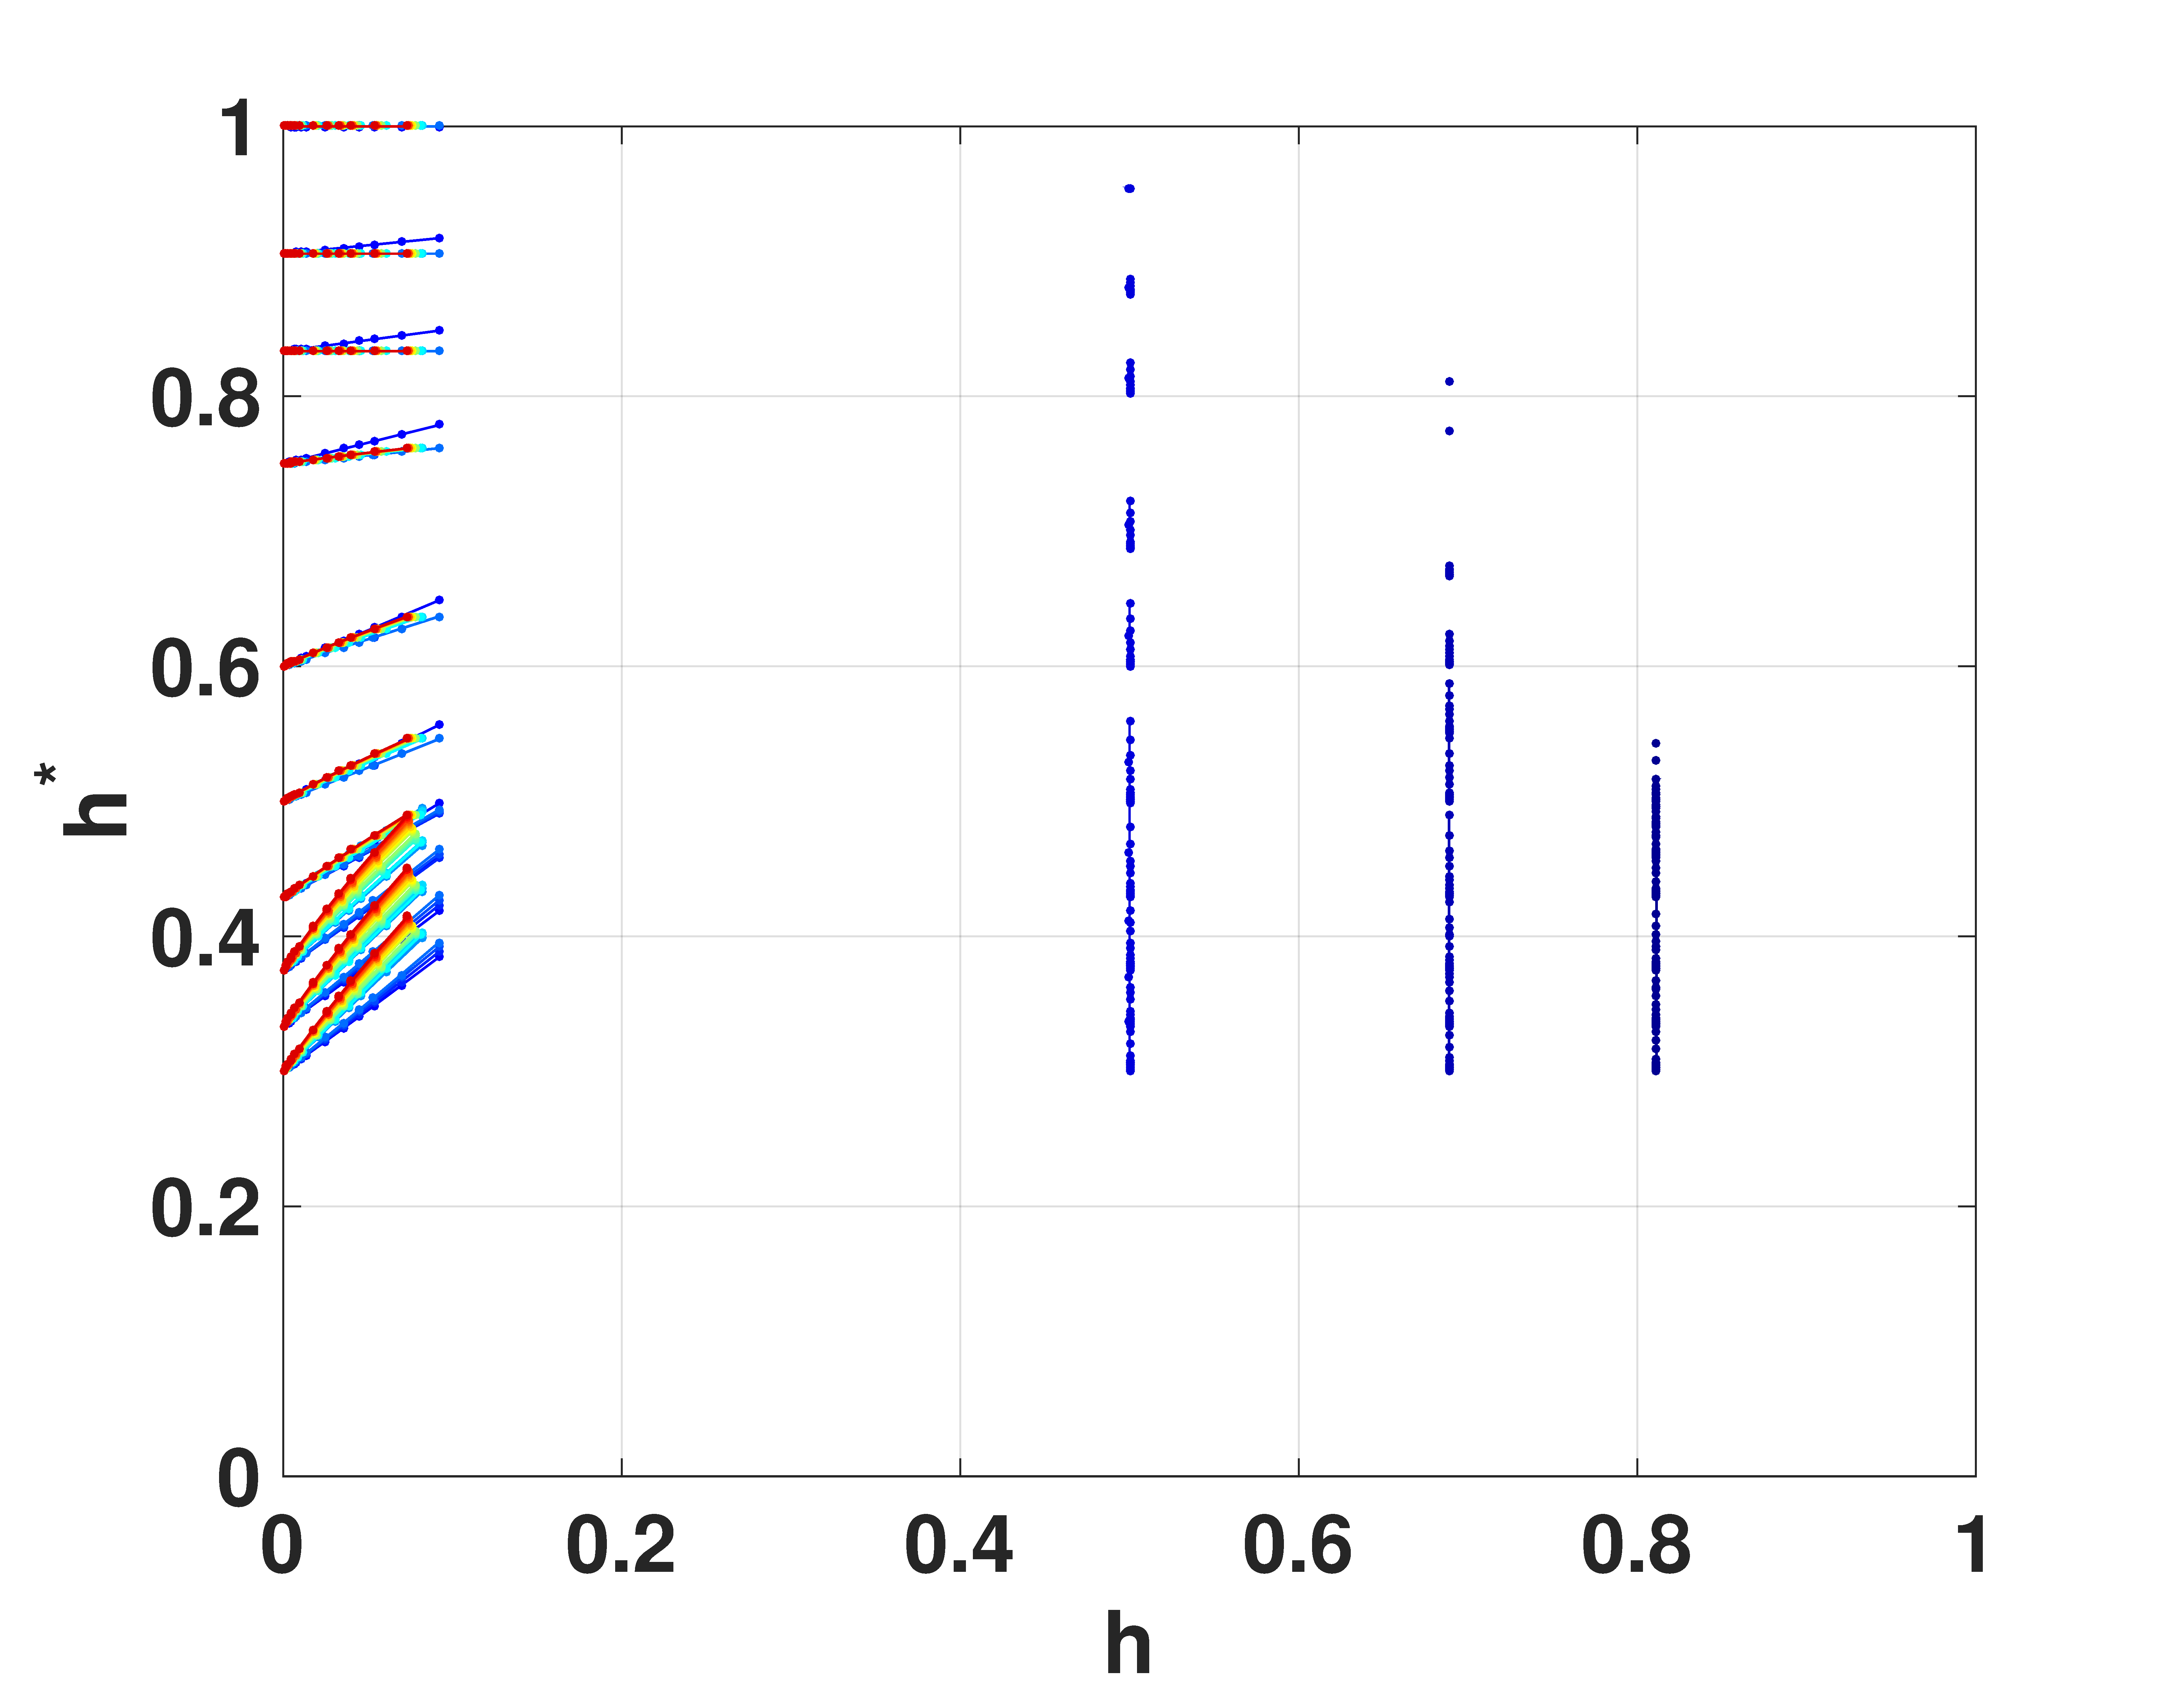
\includegraphics[width=\textwidth]{PlanoHHTodos}
	\caption{Plano doble entropía diferencial con $D$ y $W$ como parámetro.}
	\label{fig:PlanoHHTodos}
\end{figure}
%
\begin{figure}
	\centering
	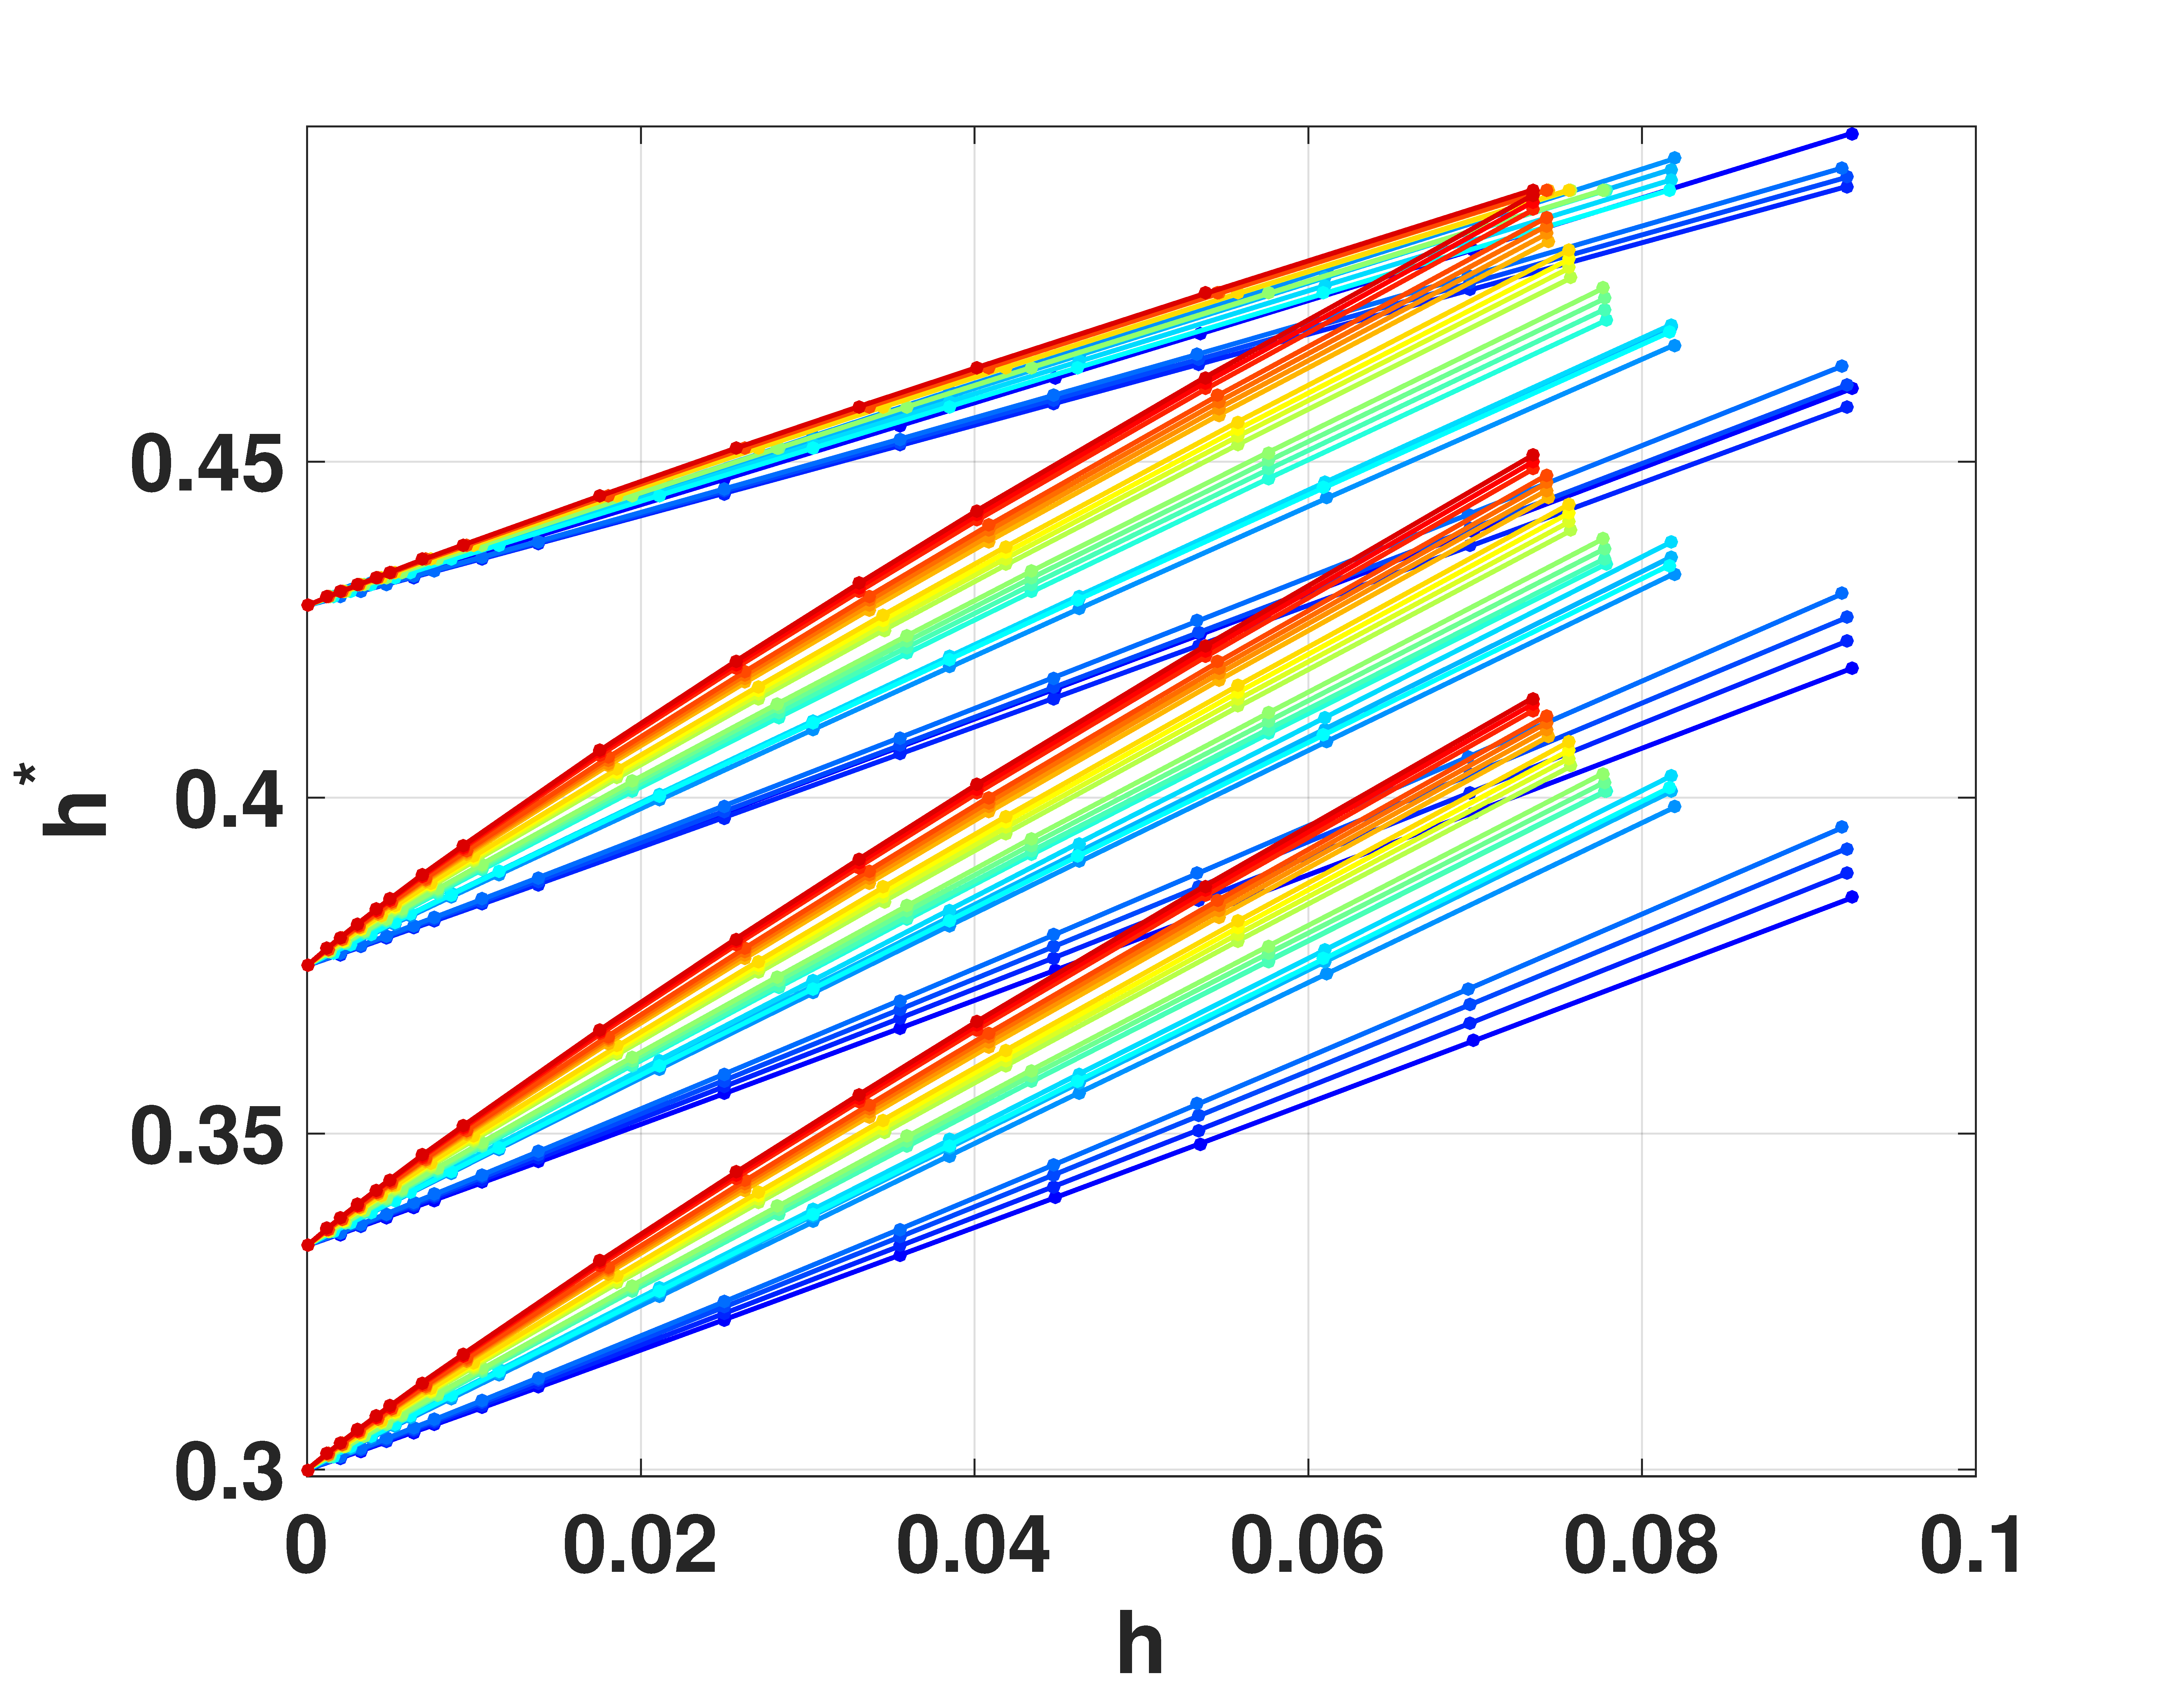
\includegraphics[width=\textwidth]{PlanoHHZoom}
	\caption{Detalle del plano doble entropía, en donde puede verse la sensibilidad como funcional de $W$ y $D$.}
	\label{fig:PlanoHHZoom}
\end{figure}
%